\documentclass[12pt,a4paper,oneside]{report}
\usepackage[margin=25mm]{geometry}
\usepackage{fontspec}
\setmainfont{Times New Roman}
\setsansfont{Arial}
\usepackage{setspace}
\onehalfspacing
\usepackage{graphicx,booktabs,longtable,tabularx,array,amsmath,amssymb,xcolor}
\usepackage[numbers,sort&compress]{natbib}
\usepackage[hidelinks,pdfpagelabels=false]{hyperref}
\usepackage{xurl}
\usepackage{bookmark}
\usepackage{fancyhdr}
\setlength{\headheight}{16pt}
\pagestyle{fancy}
\fancyhf{}
\fancyhead[L]{\small RayGuard SDP I}
\fancyhead[R]{\small Draft for team review}
\fancyfoot[C]{\thepage}
\renewcommand{\headrulewidth}{0pt}
\setlength{\emergencystretch}{3em}
\newcolumntype{Y}{>{\raggedright\arraybackslash}X}
\newcommand{\pending}[1]{\textbf{Pending verification:} #1}
\newcommand{\file}[1]{\nolinkurl{#1}}
\newcommand{\projectrecord}[1]{\textit{Project evidence:} \file{#1}.}
\graphicspath{{figures/}}
\begin{document}
\hypersetup{pageanchor=false}
\begin{titlepage}
\centering
{\Large Khalifa University\par}
\vspace{0.4cm}
{\large College of Computing and Mathematical Sciences\par}
\vspace{2cm}
{\Huge\bfseries RayGuard\par}
\vspace{0.6cm}
{\LARGE AI Powered Explosive Detection in X ray Scans\par}
\vspace{1cm}
{\Large Senior Design Project I\par}
\vspace{0.5cm}
{\large Fall 2026\par}
\vfill
\begin{minipage}{0.86\textwidth}
This report draft records the implemented single-scan prototype, research software
and collection evidence available on 21 November 2026. Full benchmark evaluation,
new training, physical scanner integration and distributed-case fusion remain
unfinished. The institutional cover format, project number, final student roster
and supervisor details require confirmation before submission.
\end{minipage}
\vfill
{\large Draft issued 21 November 2026\par}
\end{titlepage}
\hypersetup{pageanchor=true}
\pagenumbering{roman}
\chapter*{Abstract}
\addcontentsline{toc}{chapter}{Abstract}
X-ray baggage screening requires operators to interpret cluttered images in which
electronic devices can conceal suspicious material. RayGuard investigates how
object detection and an operator interface can support this inspection process
while preserving traceable evidence and explicit limitations. The SDP I work
combines a single-image prototype based on IEDXray and YOLOv10-M with preparation
for distributed component analysis across separately acquired scans. The implemented
software provides shared prediction and run contracts, dataset-audit tools, real
bounded detector execution, and a separate application for image intake, localization,
review and export. An evaluation pipeline and a general-initialization receipt
helper have been integrated; training and study orchestration exist as a software
draft. Audits identify category disagreements, cross-split duplicates, boundary
findings and incomplete physical-group provenance. A separate lab-collection
inventory contains 577 JPEG paths representing 478 distinct byte payloads, without
established quality acceptance or case labels. These findings constrain experimental
claims. Synthetic software checks and diagnostic inference demonstrate specific
implementation behavior, but do not establish full-dataset accuracy or operational
safety. The report explains requirements, models, alternatives, architecture,
implemented evidence and remaining qualification gates. Further work requires
reviewed data policies, training and evaluator integration, an owned compute pilot,
eligible benchmark reporting and validation of distributed-case reasoning.
\tableofcontents
\listoffigures
\listoftables
\chapter*{Abbreviations}
\addcontentsline{toc}{chapter}{Abbreviations}
\begin{tabular}{lp{0.78\textwidth}}
AP & Average precision\\
AR & Average recall\\
COCO & Common Objects in Context\\
GUI & Graphical user interface\\
HPC & High performance computing\\
IED & Improvised explosive device\\
IoU & Intersection over union\\
P1 / P2 & Single-scan / distributed multi-scan project workstreams\\
QC & Quality control\\
SDP & Senior Design Project\\
\end{tabular}
\clearpage
\pagenumbering{arabic}
\chapter{Introduction}
\label{ch:introduction}
\section{Problem and motivation}
Security screening of baggage involves recognizing suspicious objects under
occlusion, overlap and variable clutter. Embedded threats within electronic
devices make this problem more difficult because the host device and the
threat region are distinct concepts. A device box alone cannot establish a
threat, and a detector confidence is not an operational safety decision.
The IEDXray benchmark supplies a relevant research setting for studying these
distinctions in X-ray imagery~\citep{takele2026iedxray}.

RayGuard investigates a practical path from an authorized scan to localized
model findings, operator review and a traceable result record. The project
also considers a broader setting in which component evidence is distributed
across multiple packages. That setting requires externally justified grouping
and component labels; it cannot be obtained by arbitrarily combining unrelated
benchmark images. The second advisor meeting prioritized collection for that
distributed work while retaining a simple existing-model GUI showcase.
\projectrecord{docs/meeting_minutes/SDP_Meeting_02_Minutes_Fall_2026.md}

\section{Objectives and scope}
The original proposal calls for a 500-sample dataset with positive and negative
examples, image preprocessing, contemporary object detection, unseen-data
evaluation and a GUI supporting control and recording. The report evaluates
these objectives against actual evidence rather than treating a working screen
as completion of the full research problem.

The immediate SDP I implementation objectives are to preserve an explicit
task and category map, execute a verified detector, display original-coordinate
boxes and scores, distinguish failures from empty results, and retain provenance
through review and export. The experimental objectives are to reproduce a
supplied checkpoint's evaluation and to compare untuned and tuned models under
a controlled training-only validation design. These experiments remain distinct
from reproducing the authors' full training procedure.

\begin{table}[htbp]
\centering\small
\caption{Scope boundaries used throughout this report.}
\label{tab:scope}
\begin{tabular}{p{0.21\textwidth}p{0.31\textwidth}p{0.35\textwidth}}
\toprule Workstream & Current evidence & Remaining acceptance\\\midrule
Single-scan prototype & Bounded real inference and implemented operator workflow & Human rehearsal, eligible accuracy evaluation and full P1 decisions\\
Research software & Shared contracts, evaluator and initialization helper integrated; training draft available & Real trainer connection, reviewed data policy and qualified pilot\\
Distributed collection & Sanitized inventory and catalogue targets & QC, physical/case labels, accepted counts and collection completion\\
Distributed inference & Interface and research direction documented & Component evidence, case ground truth, fusion and evaluation\\\bottomrule
\end{tabular}
\end{table}

\section{Research background}
Baggage threat detection has been surveyed for both 2D and 3D screening
\citep{velayudhan2023survey}. Dark-field X-ray imaging combined with neural
networks has been reported to discriminate threat materials from benign
materials in proof-of-concept experiments \citep{astolfo2022darkfield}, and large
X-ray benchmarks such as SIXray address prohibited-item discovery in overlapping
images \citep{miao2019sixray}. These sources motivate the problem but do not
establish this project's performance.
The literature offers several detector architectures rather than one universal
solution. Faster R-CNN shares learned features with a region-proposal network,
providing a representative two-stage approach~\citep{ren2015faster}.
RetinaNet's focal loss addresses the imbalance encountered in dense detection,
which motivates attention to hard and rare cases without proving transfer to
this X-ray task~\citep{lin2017focal}. DETR formulates detection as set prediction
with bipartite matching~\citep{carion2020detr}; Grounding DINO incorporates grounded
pretraining for open-set detection~\citep{liu2023grounding}.
These papers motivate design alternatives, not claims that those models were
trained or evaluated by this team.

YOLOv10 proposes consistent dual assignments and an efficient architecture for
end-to-end detection~\citep{wang2024yolov10}. Its available task-matched checkpoint
and executed project backend make YOLOv10-M a practical reference for RayGuard.
This selection is based on implementation evidence and project constraints;
it does not imply that it is the highest-scoring model in the IEDXray paper.

The IEDXray release covers device, generic-explosive and specific-explosive
detection, alongside a complete annotation export. The inspected paper reports
17,360 images with a published 12,224/5,136 train/test split. Its protocol describes
separation of physical configurations and concealment setups, while the local
audit identifies four exact image-byte overlaps across the supplied splits.
The published claim and local finding must both be retained.
\projectrecord{docs/iedxray-paper-review.md}

FALCON studies component grounding and compositional reasoning within X-ray
scenes~\citep{michael2026falcon}. The project inspected its paper and release as
a research option; the release observations recorded in the repository do not
establish a running multi-package solution. Grounded component presence and
plausible language do not prove physical connectivity or dangerous assembly.
\projectrecord{docs/research.md}

\section{Literature and patent search record}
A scoping search was made on 22 November 2026 to locate related work and patents. It was limited to three web queries and is not a complete patent landscape; patent databases were not queried by classification or claim text. Table~\ref{tab:search} lists the searches, and the sources were read at the level of their abstracts and snippets.

\begin{table}[htbp]
\centering
\caption{Scoping literature and patent search, accessed 22 November 2026.}\label{tab:search}
\begin{tabular}{p{0.28\textwidth}p{0.38\textwidth}p{0.28\textwidth}}
\toprule
Query focus & Result found & Limit\\
\midrule
YOLO detectors for concealed IEDs in X-ray & Academic YOLO studies on IED replicas and small threat objects; one USPTO baggage-inspection patent that names YOLO as a detector & Snippets only; patent claims, assignee and status not verified\\
Multi-view or multi-scan fusion of detections & Multi-view detection with epipolar constraints; dual-view feature fusion; a dual-view dataset with auxiliary-view networks & Academic results only; no patent claiming cross-image detection fusion was found\\
Dark-field and multi-energy material discrimination & Reported in the supplied benchmark and survey citations & Cited through supplied papers; not independently re-read\\
Patent-focused queries (three further web searches, 22 Nov 2026) & Older related patents only: multi-sensor explosives detection with a neural network (EP0476070A1, US5153439A); X-ray and transmitted/scattered-ray baggage screening (US5600700A); dual-energy CT threat resolution (US20040258199A1); two-scanner dual-energy inspection (US9915752). No patent found for deep-learning detection of explosives hidden in modified electronics or for cross-image detection fusion & Web search snippets, not a patent-database query by classification or claim text; claims, status and assignees not verified. A Google Patents or USPTO full-text search with CPC G01V 5/20 is still required\\
Google Patents records of three hits (fetched 22 Nov 2026) & US8885938B2, Detecting concealed threats (Analogic; filed 2008, granted 2014): laptop-type object classification, neural network one option among SVM and PCA, mainly CT; KR102063859B1, airport AI baggage screening (Deepnoid; filed 2019): deep-learning X-ray classification of prohibited items; JP6678192B2, firearm detection with a neural network (Tsinghua University; filed 2018): not explosives & Status shown on the pages as active; claim text summarized by a fetch tool, not read verbatim, so claims are unverified. Not a complete database search: one of two Google Patents queries rendered; USPTO full-text search not run\\
\bottomrule
\end{tabular}
\end{table}

\section{Method and research contribution}
The engineering method begins with requirements and evidence inspection,
followed by dataset auditing, strict interfaces, bounded real inference and
application integration. Experimental preparation separates model execution
from evaluation. COCO conventions provide a common annotation and evaluation
language~\citep{lin2014coco}; the actual source category IDs remain task-specific.
For controlled improvement, Optuna supplies a framework for defining and
pruning search trials~\citep{akiba2019optuna}. Search is planned, not completed.
The selected optimization alternatives include SGD and AdamW; decoupled weight
decay motivates treating optimizer settings explicitly~\citep{loshchilov2019adamw}.

The current contribution is an auditable prototype and research-software path,
with documented findings and limitations. No new detector accuracy, tuning gain,
novel fusion method or operational safety claim is made in this draft.

\section{Repositories and individual contributions}
The shared research repository is
\url{https://github.com/abdalrahman-ismaik/SDP-I-RayGuard}.
The separate GUI repository is
\url{https://github.com/abdalrahman-ismaik/RayGuard-App}.
The application pins shared engine code through a Git submodule. GUI source
changes belong in the application checkout; its ignored predecessor is a recovery
copy. Appendix~\ref{app:contributions} records contribution evidence and outstanding
student verification. AI-assisted implementation and documentation must be disclosed
accurately; assistance does not establish a student's independent understanding.

\pending{Student-confirmed contributions, sanitized relevant prompt excerpts,
formal project number, final roster and institutional cover template. A scoped patent
search is not evidenced; this draft makes no patentability or clearance claim.}

\section{Report organization}
Chapter~\ref{ch:system} defines requirements and interfaces.
Chapter~\ref{ch:theory} explains the engineering model and evaluation quantities.
Chapter~\ref{ch:design} compares alternatives and documents constraints.
Chapter~\ref{ch:implementation} describes actual implementation and verification.
Chapter~\ref{ch:conclusions} evaluates progress and remaining work.
The appendices provide project-management evidence, requirement coverage,
risk preparation and contribution records.

\chapter{System Overview}\label{ch:system}
\section{Stakeholders and use context}
The prototype supports a human inspecting an authorized X-ray image. The
operator needs visible task identity, localized findings, usable review
controls and honest handling of missing inputs and failed execution. Students
and supervisors also need reproducible artifacts and enough provenance to
explain implementation decisions. Physical scanner integration requires a
separate observed interface handoff; public documentation and image replay do
not establish compatibility with the lab machine.

The research dataset and the lab collection serve different purposes. Public
IEDXray supports the single-scan baseline and executed generic training/evaluation.
Dismantled scans support the distributed collection workstream. Their counts
do not supply detector labels, independent cases or accepted negatives.

\section{Functional requirements}
\begin{longtable}{p{0.1\textwidth}p{0.49\textwidth}p{0.31\textwidth}}
\caption{Requirement-to-evidence map for the SDP I prototype.}\label{tab:requirements}\\
\toprule ID & Requirement & Evidence and disposition\\\midrule\endfirsthead
\toprule ID & Requirement & Evidence and disposition\\\midrule\endhead
FR1 & Accept authorized images and identify the source explicitly & Upload, folder receipt and finite replay documented; physical scanner not qualified\\
FR2 & Apply declared preprocessing consistently before inference & Canonical image and backend transforms documented; no measured enhancement benefit\\
FR3 & Detect and localize the selected task with a verified checkpoint & Generic published-test measurements in Chapter 5; device/specific diagnostic scope remains bounded\\
FR4 & Display original-coordinate boxes, scores and task identity & Shared contract and GUI implementation evidence\\
FR5 & Preserve execution failure and missing-input states & Contract/software behavior; empty results imply no benign verdict\\
FR6 & Support operator review and export traceable records & Notes, session review and JSON export; persistence beyond session remains limited\\
FR7 & Evaluate with matching ground truth and frozen settings & Generic test job 820 verified; duplicate/group limitations retained\\
FR8 & Associate distributed scans using justified case provenance & Contract direction only; case labels and fusion unfinished\\
\bottomrule
\end{longtable}

The proposal's acquisition objective remains broader than the present inventory.
The recorded catalogue plans 500 images across 125 four-bag groups. The inventory
contains 478 distinct byte payloads; the numerical difference is not an accepted
shortfall until the lab confirms round mapping and usable-count criteria.

\section{System specification}
\subsection{Inputs and outputs}
A successful scan result contains version, scan ID, execution status, original
image dimensions, model/task identity and provenance, threshold, and a detection
list. Each detection carries an ID, original-pixel corner coordinates, a category
namespace and label, a confidence value, and explicit host association where
available. An unmatched region retains no invented host link.

The run manifest binds checkpoint hash, inference-code identity, task maps,
input identities, backend settings and actual execution device. Training settings
and study records remain separate from the inference manifest. This separation
allows a candidate to be evaluated without extending every consumer with
training-specific fields.
\projectrecord{docs/contracts.md; docs/baseline-run-contract.md}

\subsection{Failure and empty-result semantics}
Execution success and detection count are separate. A successful run can contain
zero detections; it means the model reported no regions at the chosen settings.
A failed or missing scan is not an empty successful scan. Application messages
and downstream evaluation must retain this distinction. It is particularly
important for distributed cases, where a missing package cannot be treated as
evidence that a component is absent.

\subsection{Nonfunctional requirements}
Reproducibility requires matching revisions, hashes, dependency profiles and
documented settings. Local processing reduces unnecessary transfer of sensitive
imagery; raw scans, credentials and private manifests stay outside Git. Usability
requires readable overlays, keyboard review, responsive layouts and explicit
source/result identity. The team must verify these properties on the actual
presentation machine before claiming demo readiness.

Latency has at least two meanings: model execution time and total time from
accepted input to a visible completed result. Hardware, precision, batch size,
warm-up, synchronization and preprocessing/postprocessing boundaries must be
reported before comparing speeds. No stable percentile latency is inferred
from a few diagnostic samples.

\section{Acceptance boundaries}
The existing vertical slice is accepted only to its demonstrated extent.
Full P1 requires an agreed host/threat association or cascade and decision policy.
P2 additionally requires component-level evidence, justified cases and case-level
ground truth. Neither is supplied automatically by choosing a checkpoint in the
GUI. Table~\ref{tab:requirements} therefore records partial and unfinished
requirements rather than presenting all boxes as complete.

\pending{Formal supervisor acceptance of the current requirements and
mapping, current presentation-machine qualification and live scanner interface.}

\chapter{Theoretical Foundations}\label{ch:theory}
\section{Detection as the engineering model}
For a canonical RGB image $I$ of width $W$ and height $H$, a detector with
parameters $\theta$ produces a finite set
\begin{equation}
 D_\theta(I)=\{(b_i,c_i,s_i)\}_{i=1}^{n},
 \qquad b_i=(x_{1i},y_{1i},x_{2i},y_{2i}).
\end{equation}
Here $c_i$ belongs to the selected model's task namespace and $s_i$ is a model
confidence. Box corners are measured in original-image pixels with positive
width and height. The confidence is not assumed to be a calibrated probability
of a dangerous device. A task map is needed to interpret labels; a model output
index and a dataset category ID are different identifiers.

\begin{figure}[htbp]
\centering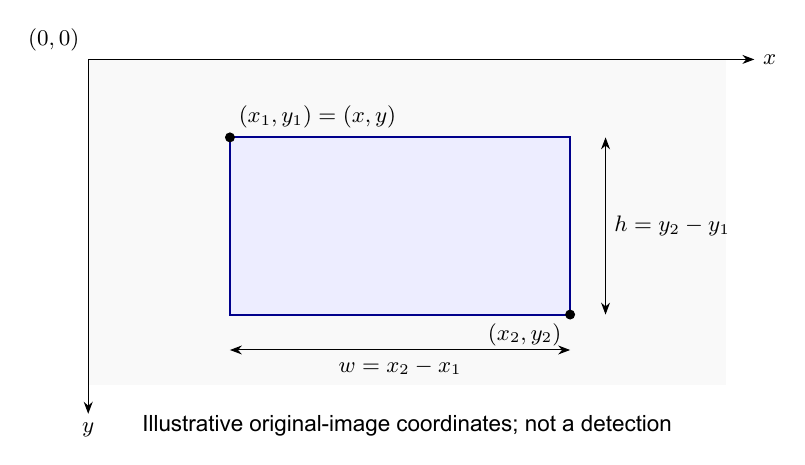
\includegraphics[width=0.82\textwidth]{coordinates.png}
\caption{Original explanatory diagram of corner and COCO box coordinates.
The rectangle is illustrative and is not a scan or model prediction.}
\label{fig:coordinates}
\end{figure}

COCO annotations use $(x,y,w,h)$. Conversion to original-pixel corners is
\begin{equation}
 (x_1,y_1,x_2,y_2)=(x,y,x+w,y+h),
\end{equation}
with inverse $(x_1,y_1,x_2-x_1,y_2-y_1)$. Any resizing or letterboxing inside the
backend must be reversed before the shared contract is emitted. The software
does not repair malformed source geometry silently. Figure~\ref{fig:coordinates}
fixes the convention used in this report.

\section{Localization and detection metrics}
For predicted region $B_p$ and reference region $B_g$, intersection over union is
\begin{equation}
 \operatorname{IoU}(B_p,B_g)=\frac{|B_p\cap B_g|}{|B_p\cup B_g|}.
\end{equation}
At a declared score threshold and matching rule, precision and recall are
\begin{equation}
 P=\frac{TP}{TP+FP},\qquad R=\frac{TP}{TP+FN}.
\end{equation}
Their denominators and undefined cases need explicit treatment. A missed
annotated threat contributes a false negative under the frozen matching rule;
an unannotated detection is not automatically a physical false alarm because
annotation completeness may itself be limited.

COCO AP@[.50:.95] summarizes detection over IoU thresholds from 0.50 to 0.95;
AP50 reports the 0.50 case, and AR summarizes recall under the evaluator's
detection limits. These definitions are implemented by the official evaluator
and must be interpreted with its settings and task maps~\citep{lin2014coco}.
The validation objective returns AP as a fraction from 0 to 1. Published tables
may display percentages; comparing them requires an explicit scale conversion.

\section{Training and validation independence}
Let $T$ be the published training image set and $E$ the published test set.
Controlled improvement requires disjoint fit and validation partitions
$T_f,T_v\subset T$ such that $T_f\cap T_v=\varnothing$ and
$T_f\cup T_v=T$, subject to the reviewed data policy. Exact duplicate bytes and
verified physical groups must not cross $T_f$ and $T_v$. A connected group may
contain several images, so a target 80/20 fraction need not be attained exactly.

The author checkpoints may have seen all published training images. Carving
validation from those images does not make them unseen for those checkpoints.
For controlled U/T experiments, both models start from general pretraining
with documented exclusion evidence and the same task-head initialization
procedure. They share the fixed partition and comparable training budget;
the tuned model's choices are selected on validation, not on the test set.

\section{Optimization and experiment identity}
The planned search objective is
\begin{equation}
 \lambda^*=\arg\max_{\lambda\in\Lambda}
 \operatorname{AP}(f_{\theta(T_f,\lambda)},T_v),
\end{equation}
where $\lambda$ denotes the declared hyperparameters. Optuna supports trial
search and pruning~\citep{akiba2019optuna}; this does not establish that an
improvement exists. Untuned and tuned inference records use distinct output
checkpoint hashes with a common starting-weight parent hash. Matching that
parent is necessary but insufficient: code, task, partition, settings, seeds
and training budgets also need review.

\section{Limits of the model}
Single-image box detection represents appearance and location. It does not
establish chemical composition, electrical connectivity or assembly intent.
FALCON's compositional formulation motivates asking about relationships, but
does not remove the need for suitable supervision and case evaluation
\citep{michael2026falcon}. RayGuard's P2 interface therefore requires external
case provenance and keeps missing scans visible. No mathematical aggregation
rule is presented here as an implemented distributed detector.

\chapter{Concept Generation and Design Evaluation}\label{ch:design}
This chapter generates alternative concepts for each part of the system, evaluates
them against stated criteria, and describes the selected design. It defines the
evaluation criteria (Section~\ref{sec:criteria}), generates and assesses the
detector concepts (Section~\ref{sec:detector}) and the system concepts
(Section~\ref{sec:sysconcepts}), presents the selected architecture
(Section~\ref{sec:architecture}), discusses pre-processing and host association
(Section~\ref{sec:preproc}), and closes with the realistic constraints, standards
and ethical considerations (Section~\ref{sec:realistic}).

%-----------------------------------------------------------------------------
\section{Evaluation Criteria}\label{sec:criteria}
Each concept was judged against the five criteria in Table~\ref{tab:criteria}.
They follow from the requirements of Chapter~\ref{ch:system}: the system must run
real models now, produce traceable results, support an operator, remain
explainable by its student contributors, and avoid claims the evidence does not
support.

\begin{table}[htbp]
\centering\tablesetup
\caption{Criteria used to evaluate design concepts.}
\label{tab:criteria}
\begin{tabularx}{\textwidth}{@{}lL{0.25\textwidth}Y@{}}
\toprule
ID & Criterion & Question asked of each concept\\
\midrule
C1 & Demonstrated compatibility & Has it been executed with a verified,
task-matched checkpoint?\\
C2 & Reproducibility & Can a run be repeated and traced to its code, weights and
settings?\\
C3 & Operator value & Does it give the operator clear, localized and honest
feedback?\\
C4 & Effort and explainability & Can the team build it in SDP~I and explain every
part?\\
C5 & Claim risk & Does it avoid results or capabilities that the evidence does not
yet support?\\
\bottomrule
\end{tabularx}
\end{table}

%-----------------------------------------------------------------------------
\section{Detector Concepts}\label{sec:detector}
The IEDXray authors supplied checkpoints for six detector families, each trained
for the device, generic-explosive and specific-explosive tasks. They cover the
main design families of Section~\ref{sec:background}: a one-stage detector
(YOLOv10-M), two-stage detectors (Faster R-CNN and Cascade R-CNN), set-prediction
transformers (DETR and the anti-overlapping variant AO-DETR) and an open-set,
text-conditioned detector (Grounding DINO)~\citep{takele2026iedxray}. All 18 files
were hashed and their metadata inspected without loading the models. The
inspection found task-pairing problems in several non-YOLO files, such as a
specific-task Faster R-CNN checkpoint whose stored class names disagree with its
configured class count, and DETR files that store 92 outputs without class names.
\projectrecord{docs/checkpoint-catalog.md}

Table~\ref{tab:detector-eval} rates the six families against the criteria. A
rating of $+$ means the criterion is satisfied on current evidence, $\circ$ that
it is partly satisfied or unknown, and $-$ that it is not satisfied. The ratings
are a qualitative design assessment based on the inspection record, not a
measured accuracy comparison.

\begin{table}[htbp]
\centering\tablesetup
\caption{Qualitative evaluation of the supplied detector families
($+$ satisfied, $\circ$ partial or unknown, $-$ not satisfied).}
\label{tab:detector-eval}
\begin{tabularx}{\textwidth}{@{}L{0.2\textwidth}cccccY@{}}
\toprule
Detector family & C1 & C2 & C3 & C4 & C5 & Basis\\
\midrule
YOLOv10-M & $+$ & $+$ & $+$ & $+$ & $+$ & All three tasks executed on CPU and
GPU; class maps inspected; no NMS step\\
Faster R-CNN & $-$ & $\circ$ & $+$ & $\circ$ & $-$ & Head and label mismatch in
the specific task; needs MMDetection\\
Cascade R-CNN & $-$ & $\circ$ & $+$ & $\circ$ & $\circ$ & Class ordering of the
specific task unverified; needs MMDetection\\
DETR & $-$ & $-$ & $+$ & $\circ$ & $-$ & 92 outputs with no stored class names\\
AO-DETR & $-$ & $\circ$ & $+$ & $-$ & $\circ$ & Requires custom modules and
mapping verification\\
Grounding DINO & $-$ & $\circ$ & $+$ & $-$ & $-$ & Text prompts and category
handling must be verified together\\
\bottomrule
\end{tabularx}
\end{table}

YOLOv10-M is the only family that satisfies every criterion and is therefore the
selected reference detector. The other families remain research comparisons; no
local result is claimed for them. This selection reflects implementation evidence
and does not imply that YOLOv10-M scores highest in the IEDXray benchmark.

%-----------------------------------------------------------------------------
\section{System Concepts}\label{sec:sysconcepts}
Table~\ref{tab:alternatives} lists the alternatives considered for the other
design decisions and the reason for each selection. Each decision is also
recorded in the project's decision log.
\projectrecord{docs/decisions.md}

\begin{table}[htbp]
\centering\tablesetup
\caption{System design alternatives and the selected concept.}
\label{tab:alternatives}
\begin{tabularx}{\textwidth}{@{}L{0.17\textwidth}L{0.24\textwidth}L{0.2\textwidth}Y@{}}
\toprule
Decision & Alternatives & Selected & Reason\\
\midrule
Pipeline layout & Full-image detection; host-crop cascade & Full-image detection
& Avoids losing threats when a host box is missed (C3, C5); association rule
remains open\\
Image input & Manual upload; watched folder; scanner SDK & Upload, watched folder
and replay & Reversible and needs no scanner access; an SDK requires an observed
hardware interface (C1, C5)\\
Execution boundary & Model in main environment; isolated runtime & Isolated
runtime & Keeps the locked CPU tools small and each task's runtime qualified
(C2, C4)\\
Application stack & Desktop wrapper; cloud service; local web app &
React/TypeScript front end with local FastAPI & Runs locally without uploading
scans; familiar tools (C3, C4)\\
Interface between parts & Ad-hoc outputs; versioned contract & Versioned JSON
contract & Separates empty, missing and failed results; testable (C2, C3)\\
Study initialization & Continue author checkpoint; general pre-training &
General pre-training & The author checkpoint may have seen the validation images
(C5)\\
\bottomrule
\end{tabularx}
\end{table}

%-----------------------------------------------------------------------------
\section{Selected Architecture}\label{sec:architecture}
Figure~\ref{fig:architecture} shows the selected architecture. The application
and the research engine live in separate repositories. The operator interface and
a local API handle interaction; the engine, pinned as a Git submodule, supplies the
contracts, the model catalogue and the inference tools. The selected model runs in
its own qualified environment, and the API validates every returned scan result
before the interface displays it. The research path, which trains and validates
new candidates, was qualified and executed on the HPC cluster for the generic
study of Section~
ef{sec:results}; its checkpoints are not yet loaded by the
application.
\projectrecord{docs/architecture.md}

\begin{figure}[htbp]\centering
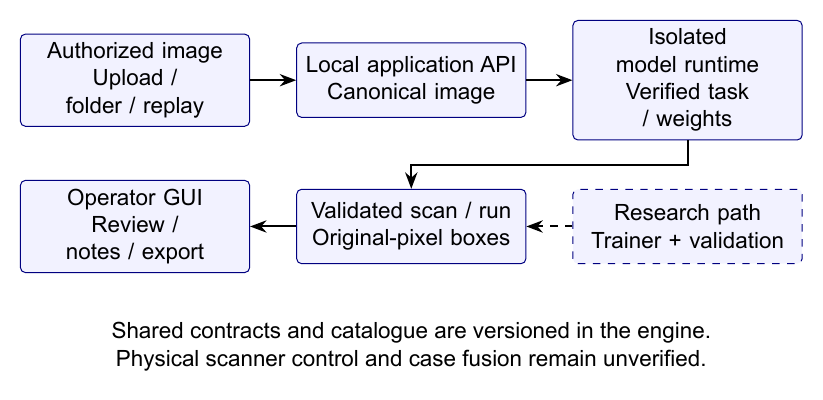
\includegraphics[width=\textwidth]{architecture.png}
\caption{Selected system architecture. Solid arrows show the implemented prototype
path; the dashed research path was executed on HPC for the generic study but is
not yet connected to the application.}
\label{fig:architecture}
\end{figure}

Two design rules keep the data consistent. First, the source image, its
canonically oriented copy and the original-coordinate predictions stay linked
throughout the pipeline. Second, operator viewing adjustments change only the
display and never become model pre-processing. Session history and saved evidence
also have different lifetimes: the visible session list may reset, while the
private run records remain.

%-----------------------------------------------------------------------------
\section{Pre-processing and Host Association}\label{sec:preproc}
The proposal asks for image enhancement such as noise reduction and contrast
adjustment. A filter applied before inference changes the input distribution that
the checkpoint was trained on, and may lower accuracy even if the image looks
clearer to a person. The design therefore applies only the checkpoint's own
normalization before inference and offers viewing adjustments, such as contrast, in
the display. Any enhancement before inference should be compared against an
identity reference under the validation protocol of Chapter~\ref{ch:theory}; no
benefit is claimed here.

The relation between a threat region and its host device was considered in two
forms. A \emph{host-crop cascade} first detects devices and then searches inside
each crop, which removes background but loses any threat whose host was missed;
it also needs rules for overlapping hosts, padding and regions crossing the crop
edge. \emph{Full-image detection} avoids that failure mode but still needs a
justified rule linking each threat to a host. The separate device and explosive
annotations of IEDXray do not decide between them, so the decision is left open
and the scan result records an explicit null association when the link is unknown.

%-----------------------------------------------------------------------------
\section{Realistic Constraints, Standards and Ethics}\label{sec:realistic}

\subsection{Realistic Constraints}
Table~\ref{tab:constraints} summarizes the constraints that shaped the design.

\begin{table}[htbp]
\centering\tablesetup
\caption{Realistic design constraints and the design response to each.}
\label{tab:constraints}
\begin{tabularx}{\textwidth}{@{}L{0.17\textwidth}YY@{}}
\toprule
Constraint & Situation & Design response\\
\midrule
Economic & Proposal budget of 1,000~AED; GPUs provided by the CVML laboratory &
Open-source software only; no paid services\\
Compute & HPC access with a time limit per job; runtime unknown at design time
& A bounded pilot before the search; measured study used 10~h of GPU time\\
Data & Limited real threat data; test split must stay untouched & Audit before
use; group-preserving partitions; new laboratory collection\\
Safety & Threat items are laboratory simulants; scanner operated in the
laboratory & Collection only under laboratory procedures\\
Privacy and security & Scans and credentials are sensitive & Local processing;
scans kept off the public repository\\
Time & One semester with five students & Small, explainable components with
clear interfaces\\
\bottomrule
\end{tabularx}
\end{table}

\subsection{Standards}
The design follows the COCO conventions for annotations and metrics and a versioned
JSON interface for interoperability between components~\citep{lin2014coco}. These
are technical conventions, not certification under aviation, radiation-safety or
security-screening standards; a deployed screening aid would require such
certification. The inspected IEDXray release contains processed RGB images rather
than the raw dual-energy signal, so material classes are not inferred from the
display colours.

\subsection{Ethics and Sustainability}
The main risks of the system are missed detections, operator over-reliance,
leakage of private data and misleading demonstrations. The design responds with
explicit error states, known misses kept in the record, provenance on every result
and the position of the system as an aid to a human operator. Laboratory work
follows the supervisor's scanner and safety procedures. On the computational side,
the study uses a measured pilot, a bounded number of trials and reuse of valid
results; no energy saving is claimed without measurement.

The selected design is implemented as described in Chapter~\ref{ch:implementation}.

\chapter{Implementation and Fabrication}\label{ch:implementation}
RayGuard involves no physical hardware build. Its fabrication-equivalent work is
the construction of the software pipeline and operator application, the
collection of the X-ray dataset, and the verification records that support each
claim. This chapter describes the implemented software (Section~\ref{sec:software}),
the dataset audit and collection (Section~\ref{sec:data}), the verification
results (Section~\ref{sec:verification}), the evaluation protocol and the executed
fine-tuning study (Section~\ref{sec:protocol}), the resulting prototype detection
results (Section~\ref{sec:results}), a walkthrough of the application
(Section~\ref{sec:walkthrough}), and the remaining application acceptance
(Section~\ref{sec:acceptance}).

%-----------------------------------------------------------------------------
\section{Software Implementation}\label{sec:software}

\subsection{Implemented Components}
The software is split between the research repository, which holds the shared
engine, contracts and research tools, and the application repository, which holds
the operator interface. Table~\ref{tab:components-sw} lists the components, the
pull request or commit through which each entered the code base, and the level of
evidence behind it.

\begin{table}[htbp]
\centering\tablesetup
\caption{Implemented software components.}
\label{tab:components-sw}
\begin{tabularx}{\textwidth}{@{}L{0.22\textwidth}YL{0.2\textwidth}L{0.17\textwidth}@{}}
\toprule
Component & Function & Integration & Evidence\\
\midrule
Audit tools & Decode images and check COCO annotations, splits and box geometry &
Research repository, \file{main} & Executed on IEDXray\\
Run contract and baseline adapter & Validate saved predictions against the run
manifest and the task class map & PRs~\#17, \#19 & Synthetic tests; CI\\
Evaluator & Convert boxes to COCO format and compute AP and AR under a frozen
protocol & PR~\#18 (\file{9350482}) & Synthetic tests; CI\\
Initialization receipt & Hash the YOLOv10-M starting weights and reject a
mismatch & PR~\#21 (\file{29d6d0f}) & Synthetic tests; CI\\
Box repair & Clamp five sub-pixel training boxes in a derived copy with a change
record & PRs~\#22, \#24 & Executed on the training exports\\
Training workflow & Data checks, shared partition, Optuna search, Slurm jobs,
checkpoint provenance and qualification & PR~\#25 & Executed on HPC (T41)\\
Frozen test runner & Evaluate a preselected checkpoint pair on the published test
set under a hashed plan & PR~\#25 & Executed on HPC (job 820)\\
Operator application & Image intake, localization, review, notes and export &
RayGuard-App & Executed on real scans\\
\bottomrule
\end{tabularx}
\floatnote{Integration record and evidence level on 23~November~2026.}
\end{table}

\subsection{Operator Application}
The operator application, RayGuard-App, pins an explicit revision of the research
engine as a Git submodule. It accepts images by upload, by receipt of completed
images in a watched folder, and by replay of a finite set of published images. For
the selected task it displays the detector's boxes and scores in original image
coordinates, provides viewing adjustments, links each finding to its region, and
lets the operator add notes, record a review decision and export the result as
JSON with its provenance. The application does not connect directly to a physical
scanner and does not provide persistent case management.

\subsection{Evaluation and Run Contracts}
The baseline adapter accepts saved predictions only when they match the identity
in the run manifest and the class map of the task. The evaluator converts
original-pixel corner boxes $(x_1,y_1,x_2,y_2)$ to COCO $(x,y,w,h)$ format and
keeps the dataset's own category identifiers, including the generic category
zero. It refuses a full evaluation when any required scan failed or is missing,
unless an explicitly labelled subset mode is requested. An approved protocol
requires a hash of the ground-truth file, and a matched comparison requires
identical, clean inference code for both models.

The validation objective added in PR~\#18 checks the identities of the checkpoint
and annotation files, the task, the requested image coverage and the frozen
evaluator settings, and returns AP on a 0--1 scale. The caller remains responsible
for computing real file hashes and binding predictions to the checkpoint that
produced them; a recorded partition hash alone does not prove the partition.

\subsection{Training Workflow}
The initialization receipt (PR~\#21) hashes a local copy of the official
YOLOv10-M starting weights and rejects a mismatch without loading the model.
Documentary evidence and the COCO metadata support its use as general
pre-training; this does not prove the training contents or verify the copy on
the high-performance computing (HPC) cluster; the copy used for training was
re-hashed on the cluster before each run.

The training workflow (PR~\#25) runs each stage in an isolated Python~3.12
environment with the pinned YOLOv10 fork on one NVIDIA H100 NVL GPU allocated
through Slurm. Every stage writes a receipt that binds the code, the starting
weights, the data bundle and the settings, and the command-line tools refuse to
start without an explicit execution authorization. Bounded pilot jobs first
established forward and backward passes, checkpoint saving and reloading, the
class mapping, validation and the runtime per epoch. Figure~\ref{fig:experiments}
shows the intended separation between reproduction of the supplied checkpoint and
the controlled study; the study actually executed is described in
Section~\ref{sec:protocol}.

\begin{figure}[htbp]\centering
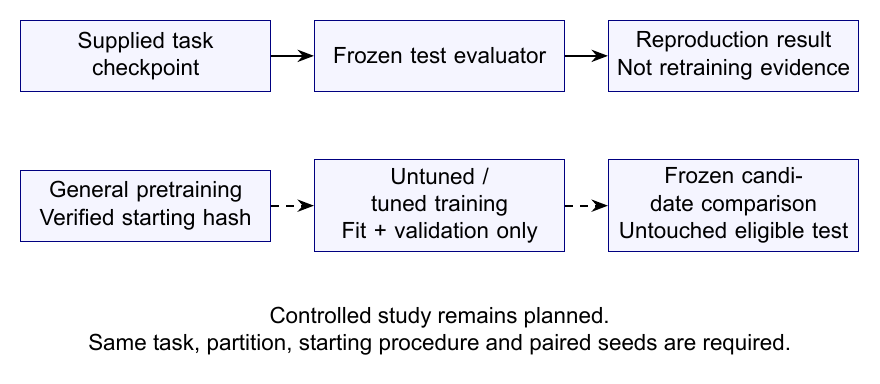
\includegraphics[width=\textwidth]{experiments.png}
\caption{Experiment design.}
\label{fig:experiments}
\floatnote{The upper path reproduces the supplied checkpoint; the lower path is the controlled study, executed in reduced form as shown in Figure~\ref{fig:t41flow}.}
\end{figure}

%-----------------------------------------------------------------------------
\section{Dataset Inspection and Collection}\label{sec:data}

\subsection{IEDXray Audit}
Before any model output was trusted, the supplied IEDXray release was audited.
The audit decoded all 17,360 images and inspected eight annotation files. A
second, read-only preflight of the authorized local copies was run for the T41
study. Table~\ref{tab:audit} summarizes the findings of both. Small numerical
excursions of box coordinates are qualitatively different from semantic label
disagreements and are reported separately. Neither check authorizes a global
label swap or silent clipping of boxes, and the published test data and original
annotations were left unchanged.
\projectrecord{docs/iedxray-audit.md; docs/iedxray-paper-review.md; docs/progress.md}

\begin{table}[htbp]
\centering\tablesetup
\caption{Findings of the IEDXray audit and the T41 preflight.}
\label{tab:audit}
\begin{tabularx}{\textwidth}{@{}YrL{0.36\textwidth}@{}}
\toprule
Finding & Value & Implication\\
\midrule
Images decoded (audit) & 17,360 & Release readable in full\\
Training / test images (preflight) & 12,224 / 5,136 & Matches the published
split\\
Device-label disagreements between exports & 4,955 & Label source must be fixed
per task\\
Distinct boundary findings (audit) & 13 & Reviewed repair needed, no silent
clipping\\
Out-of-image boxes in training exports (preflight) & 5 & Largest overshoot
0.0002745~px\\
Exact-duplicate groups within training & 5 & Keep duplicates in one partition\\
Exact-duplicate groups within test & 112 & Report; test split not altered\\
Exact-byte overlaps between training and test & 4 & Exclude from derived
training data\\
Verified physical-group identifiers & None & Group independence unknown\\
\bottomrule
\end{tabularx}
\end{table}

The preflight findings are bound to the inventory hash
\file{4e5ff81087cc7a7b0bcbbf1abf45806e96ebd7936aca35b583d7f33e471ce9f7}.
They describe the local authorized copies, not an approved partition. The data
owner must confirm the matching inventory on the HPC cluster before derived
training data are created. No repair, partition, training or evaluation was
performed in this step.

\subsection{Collection of Positive X-ray Scans}\label{sec:collection}
The proposal requires a dataset of 500 samples containing positive and negative
scans. The positive scans were collected by the five students in the CVML
laboratory on a dual-energy baggage scanner supplied by Secure Life Group (SLG).
Collection followed the laboratory's multi-bag catalogue, which fixes for every
scan the bag, the threat component and the clutter around it. Each group of the
catalogue occupies four bag slots (A--D), and each slot holds one registered
component from a different family, so that one group distributes a complete set
of IED components over four separate bags (Table~\ref{tab:components}). This
design serves the single-scan task now and the distributed task of SDP~II later.
\projectrecord{docs/meeting_minutes/follow-up-collection-2026-09-28.md}

\begin{table}[htbp]
\centering\tablesetup
\caption{Component families of the collection catalogue.}
\label{tab:components}
\begin{tabularx}{\textwidth}{@{}L{0.24\textwidth}L{0.16\textwidth}Y@{}}
\toprule
Component family & Item codes & Role in an IED\\
\midrule
Explosive simulant & E1--E4 & Main charge\\
Detonator simulant & D1--D3 & Initiator\\
Battery & B1--B3 & Power source\\
Wire & W1--W2 & Electrical connection\\
\bottomrule
\end{tabularx}
\floatnote{All items are labelled laboratory items; explosive and detonator items are simulants.}
\end{table}

Table~\ref{tab:catalogue} summarizes the structure of the catalogue. Every student
was assigned 25 groups (100 bags) over two sessions, so the five students together
cover 125 groups and 500 bag configurations. Each component family appears in
125 configurations, and the catalogue balances five clutter levels and four target
orientations. A structural check of the catalogue confirmed that every group has
four bags with one target from each family.

\begin{table}[htbp]
\centering\tablesetup
\caption{Structure of the Round~1 collection catalogue.}
\label{tab:catalogue}
\begin{tabularx}{\textwidth}{@{}L{0.3\textwidth}Y@{}}
\toprule
Element & Specification\\
\midrule
Configuration group & Four bags (A--D); one explosive simulant, one battery, one
detonator simulant and one wire, each in its own bag with specified clutter\\
Allocation per student & Session~A: 12 groups (48 bags); Session~B: 13 groups (52
bags); 25 groups (100 bags) in total\\
Whole catalogue & 125 groups, 500 bag configurations, 125 per component family\\
Clutter levels & L1--L5, 25 groups (100 bags) each\\
Target orientations & O1--O4, 125 targets each\\
Item variants & All twelve variants of Table~\ref{tab:components}\\
\bottomrule
\end{tabularx}
\end{table}

The collection activity ran from 28~September to 4~November~2026, as reported by the
team. The scan files in the laboratory snapshot are dated 29~September to
9~October~2026. The sessions followed the
schedule agreed with the laboratory (Appendix~\ref{app:management}). The team
completed the 500 catalogue configurations of Round~1. Table~\ref{tab:collection}
gives the snapshot of the laboratory computer taken on 14~November~2026, which
holds 478 distinct image files. The remaining 22 scans are not part of that
snapshot. The snapshot also contains 99 exact copies of existing images in one
storage folder; these are not counted as scans. All 577 files in the snapshot
decoded without error.
\projectrecord{docs/collection-progress-2026-11-14.md}

\begin{table}[htbp]
\centering\tablesetup
\caption{Distinct image files per student.}
\label{tab:collection}
\begin{tabularx}{\textwidth}{@{}L{0.3\textwidth}rY@{}}
\toprule
Student & Distinct files & Scan dates (files)\\
\midrule
Abd Alrahman Ismaik & 142 & 30 Sep (92), 5 Oct (34), 9 Oct (16)\\
Faisal Daoud Alzarooni & 124 & 1 Oct (72), 8 Oct (52)\\
Ahmed Almansoori & 100 & 29 Sep (24), 6 Oct (41), 9 Oct (35)\\
Ali Arif Saeed Alshamsi & 61 & 30 Sep (21), 1 Oct (16), 9 Oct (24)\\
Mohammad Arwani & 51 & 29 Sep (32), 6 Oct (19)\\
\midrule
Total in snapshot & 478 & 29 Sep -- 9 Oct 2026\\
\bottomrule
\end{tabularx}
\floatnote{Laboratory snapshot of 14~November~2026, with the scan dates taken from the file names. The snapshot does not contain all 500 collected scans.}
\end{table}

\subsection{Negative Scans}
Negative (threat-free) scans were collected by the CVML laboratory on the same
SLG-supplied scanner, with assistance from the team. The set contains about
7,000 scans and was shared with the team by the laboratory. The count is
approximate and is reported by the team; the set has not yet been inventoried in
the project repository.

\subsection{Data Handling and Remaining Work}
All scans remain on the laboratory computer. Per-image manifests are kept privately,
and no scan is stored in the public repository. Before the collected data can be
used for training, three steps remain: quality control of each scan, bounding-box
annotation of the targets, and recording of the verified group of each bag so that
related scans stay in the same data split. These steps prepare the data for model
training and for the distributed work of SDP~II.

%-----------------------------------------------------------------------------
\section{Verification Results}\label{sec:verification}

\subsection{Software Checks}
The software is verified at two levels. Automated tests exercise the contracts
and failure handling on synthetic fixtures; they establish software behaviour,
not model accuracy. Table~\ref{tab:checks} lists the checks recorded during
integration on 21~November~2026. The evaluation-enabled run uses the locked root
environment with the evaluator dependencies added:
\begin{center}\small
\texttt{uv run -{}-locked -{}-with-requirements environments/evaluation.in python -m pytest}
\end{center}
Test counts depend on the revision checked and are not a measure of product
quality.

\begin{table}[htbp]
\centering\tablesetup
\caption{Software checks recorded during integration.}
\label{tab:checks}
\begin{tabularx}{\textwidth}{@{}L{0.24\textwidth}L{0.24\textwidth}Y@{}}
\toprule
Checked revision & Result & Scope\\
\midrule
PR~\#18 head \file{6edcd68} & Ruff passed; 273 tests passed & Windows, evaluation
dependencies enabled\\
PR~\#21 head \file{3b5fa3a} & Ruff passed; 286 tests passed & Includes the
integrated evaluator and initialization receipt\\
PR~\#24 merged head \file{87094b1} & Ruff passed; 529 passed, 3 skipped &
Box-repair fixes on top of PR~\#25\\
PR~\#25 head \file{950ea84} & Ruff passed; 525 passed, 3 skipped & Training,
tuning and frozen-test software\\
Required CI & Ubuntu and Windows checks passed & Hosted CPU checks before merge;
no GPU or accuracy evidence\\
\bottomrule
\end{tabularx}
\floatnote{Recorded 21--23~November~2026. All tests use synthetic fixtures.}
\end{table}

\subsection{Diagnostic Inference}
Real inference is a separate level of evidence. The first generic-explosive run
executed the supplied checkpoint on three inspected images on CPU and recorded a
missed modified laptop in the test set; this miss is retained as a known failure.
Later application records describe bounded CPU and CUDA runs for all three
YOLOv10-M tasks. These runs establish that the models execute correctly in the
pipeline; they do not measure benchmark accuracy.

%-----------------------------------------------------------------------------
\section{Evaluation Protocol and Executed Study}\label{sec:protocol}

\subsection{Comparison Modes}
The evaluator supports two comparison modes. A baseline--candidate comparison
measures a tuned model against the supplied checkpoint. A common-parent comparison
measures untuned and tuned models trained from the same starting weights, without
treating one as initialized from the other. A difference between two models is
interpreted as a controlled result only when it is accompanied by training
receipts, paired seeds, the partition identity and comparable training budgets.
The study reported here is a common-parent comparison.

\subsection{Data Policy}
The data policy merged in PR~\#22 and amended in PR~\#25 preserves the published
test split and keeps exact-byte duplicates on the same side of a training-derived
partition. No verified physical groups are available, so that partition is
labelled exploratory and physical independence is not claimed. Five training
boxes that extend less than 0.001~pixels outside their image are clamped in a
derived copy with a change record; the source annotations are never edited, the
published test annotations are never repaired, and larger excursions stay
blocked. The repair accepts only the two published training exports, identified
by their file and content hashes. The shared seed-17 partition contains 9,779
fit images and 2,445 validation images, with every task class on both sides.

\subsection{Executed Study Design}
To fit the report deadline, the owner reduced the original 20-attempt,
three-seed design to the generic-explosive study summarized in
Table~\ref{tab:study} and Figure~\ref{fig:t41flow}. The untuned control used SGD
with an initial learning rate of 0.001, a final learning-rate fraction of 0.01,
weight decay 0.0005 and no mosaic augmentation. The search sampled these four
values; Table~\ref{tab:hyper} compares the control with the selected candidate.
Both 100-epoch confirmations started independently from the same verified
general YOLOv10-M weights, not from a search checkpoint.

\begin{table}[htbp]
\centering\tablesetup
\caption{Design of the executed reduced fine-tuning study (T41).}
\label{tab:study}
\begin{tabularx}{\textwidth}{@{}L{0.26\textwidth}Y@{}}
\toprule
Element & Setting\\
\midrule
Task & Generic explosive detection, one class (category 0)\\
Starting weights & Official general YOLOv10-M (66,924,323 bytes), hash-verified\\
Data & Shared seed-17 partition: 9,779 fit and 2,445 validation images\\
Search & Six attempted configurations of 30 epochs, including the untuned control;
failed attempts count\\
Selection & Validation AP@[.50:.95] after each epoch; test data never used\\
Confirmation & Control and best candidate, 100 epochs each, seed 17\\
Fixed settings & Image size 640, batch 32, FP32, two data-loader workers\\
Hardware & One NVIDIA H100 NVL, four CPUs, 32~GB memory, four-hour job limit\\
Deferred & Specific-explosive task; seeds 29 and 43; full 20-attempt search\\
\bottomrule
\end{tabularx}
\end{table}

\begin{figure}[htbp]\centering
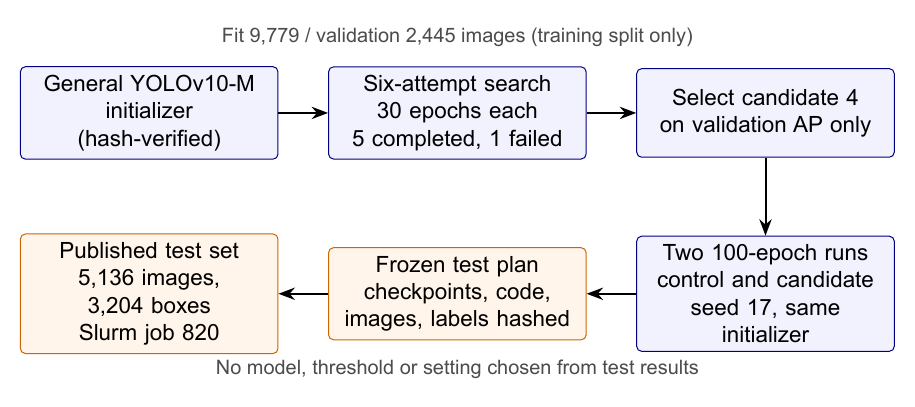
\includegraphics[width=\textwidth]{t41-flow.png}
\caption{Executed T41 study.}
\label{fig:t41flow}
\floatnote{Blue stages use the training split only; orange stages touch the published test set once, after both checkpoints were fixed.}
\end{figure}

\begin{table}[htbp]
\centering\tablesetup
\caption{Hyperparameters of the control and the candidate.}
\label{tab:hyper}
\begin{tabular}{@{}lrr@{}}
\toprule
Hyperparameter & Untuned control & Candidate 4\\
\midrule
Optimizer & SGD & SGD\\
Initial learning rate & 0.001 & 0.000394\\
Final learning-rate fraction & 0.01 & 0.0249\\
Weight decay & 0.0005 & 0.000133\\
Mosaic probability & 0.0 & 0.394\\
\bottomrule
\end{tabular}
\floatnote{Untuned control and selected search candidate. All other settings are identical.}
\end{table}

%-----------------------------------------------------------------------------
\section{Prototype Results: Generic Explosive Detection}\label{sec:results}
This section reports the first measured results of the RayGuard detector. They
come from saved predictions whose metrics a separate process recomputed exactly,
and they are descriptive results for one preselected pair of models trained with
one seed.

\subsection{Search and Confirmation}
Table~\ref{tab:t41jobs} lists every training job. Attempt~0, the untuned
configuration, failed during validation at epoch~6: the pinned detector clipped
predicted boxes lying wholly outside the image to zero area, which the evaluator
rejected. A scoped correction now keeps the original box for such predictions,
and diagnostic and qualification jobs (756 and 757) confirmed that all earlier
predictions and scores were unchanged. The failed attempt still counts against the
budget. The five completed attempts reached validation AP between 86.11\% and
86.99\% after 30 epochs (Figure~\ref{fig:t41search}); attempt~4 was selected.
Successful jobs used 9~h~57~min of GPU time, or 10~h~09~min including the
failure, and every job stayed within its four-hour limit.

\begin{table}[htbp]
\centering\tablesetup
\caption{T41 training jobs.}
\label{tab:t41jobs}
\begin{tabular}{@{}llllr@{}}
\toprule
Stage & Slurm job & Outcome & Elapsed & Val.\ AP\\
\midrule
Search attempt 0 (control) & 755 & Failed at epoch 6 & 0:11:53 & --\\
Search attempt 1 & 758 & 30 epochs & 0:52:41 & 86.81\\
Search attempt 2 & 759 & 30 epochs & 0:52:29 & 86.11\\
Search attempt 3 & 762 & 30 epochs & 0:52:23 & 86.26\\
Search attempt 4 (selected) & 764 & 30 epochs & 0:52:35 & 86.99\\
Search attempt 5 & 767 & 30 epochs & 0:52:34 & 86.18\\
Control confirmation & 770 & 100 epochs; epoch 68 kept & 2:47:35 & 87.71\\
Candidate confirmation & 819 & 100 epochs; epoch 84 kept & 2:46:49 & 87.48\\
\bottomrule
\end{tabular}
\floatnote{Validation AP@[.50:.95] in percent on the training-split validation set.}
\end{table}

\begin{figure}[htbp]\centering
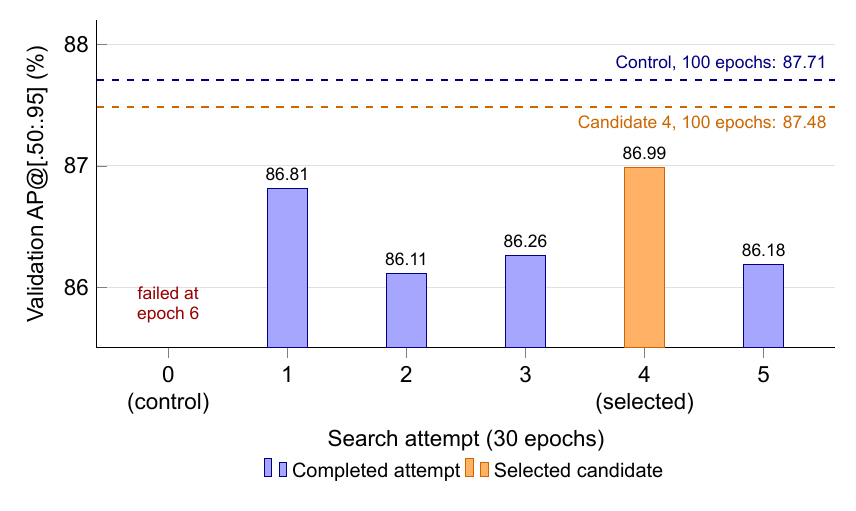
\includegraphics[width=0.9\textwidth]{t41-search.png}
\caption{Validation AP of the search attempts.}
\label{fig:t41search}
\floatnote{Six attempts after 30 epochs and two 100-epoch confirmations (dashed). Attempt 0 failed and has no score.}
\end{figure}

In confirmation, the candidate scored 0.22 percentage points below the control
on validation. The search is too small to show convergence of the Bayesian
sampler: the five sampled attempts all fall within its five random startup
trials. On validation alone,
therefore, tuning showed no benefit.

Figure~\ref{fig:t41curves} shows validation AP after every epoch of the two
confirmation runs. The candidate learned faster during roughly the first 40
epochs, but both runs levelled off at about 87\% after epoch~50 and remained
there; the selected epochs are the maxima of their runs. The plateau indicates
that further epochs alone would not have raised validation AP.

\begin{figure}[htbp]\centering
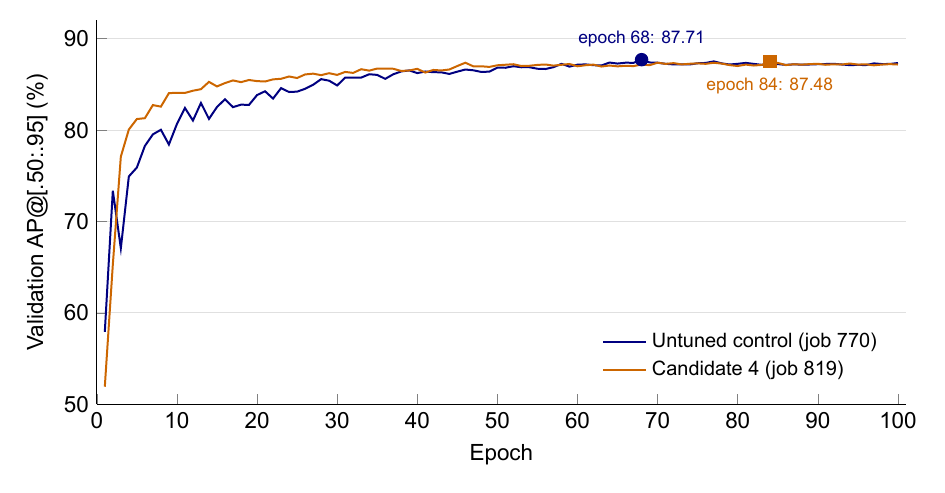
\includegraphics[width=0.95\textwidth]{t41-curves.png}
\caption{Validation AP per epoch of the confirmation runs.}
\label{fig:t41curves}
\floatnote{Two 100-epoch runs; markers show the selected epochs.}
\end{figure}

\subsection{Frozen Test Results}
Before any test image was processed, a test plan fixed the two checkpoints, the
code, the hash of every test image, the original annotations and all settings.
Slurm job~820 then evaluated both models on all 5,136 published test images and
3,204 annotated boxes in 1~min~27~s. Inference used batch size one, FP32, image
size 640, a score floor of 0.001 and at most 300 detections per image; COCO
metrics were computed with pycocotools~2.0.11~\citep{lin2014coco}.
Table~\ref{tab:t41test} gives the results and Figures~\ref{fig:t41test}
and~\ref{fig:t41size} plot them.

\begin{table}[htbp]
\centering\tablesetup
\caption{Frozen test results of the generic detector.}
\label{tab:t41test}
\begin{tabular}{@{}lrrr@{}}
\toprule
Metric & Untuned control & Candidate 4 & Difference\\
\midrule
AP@[.50:.95] & 41.59 & 48.05 & $+6.46$\\
AP@.50 & 63.40 & 66.54 & $+3.14$\\
AP@.75 & 42.29 & 52.35 & $+10.06$\\
AR@1 & 47.33 & 51.91 & $+4.57$\\
AR@100 & 49.26 & 53.27 & $+4.01$\\
\midrule
AP small / medium / large & 33.49 / 35.87 / 47.47 & 27.05 / 43.57 / 53.57 & \\
AR small / medium / large & 50.70 / 46.98 / 51.24 & 37.89 / 51.43 / 56.68 & \\
\midrule
Validation AP@[.50:.95] & 87.71 & 87.48 & $-0.22$\\
\bottomrule
\end{tabular}
\floatnote{Values in percent on the published test set. These are project measurements, not the scores published for IEDXray.}
\end{table}

\begin{figure}[htbp]\centering
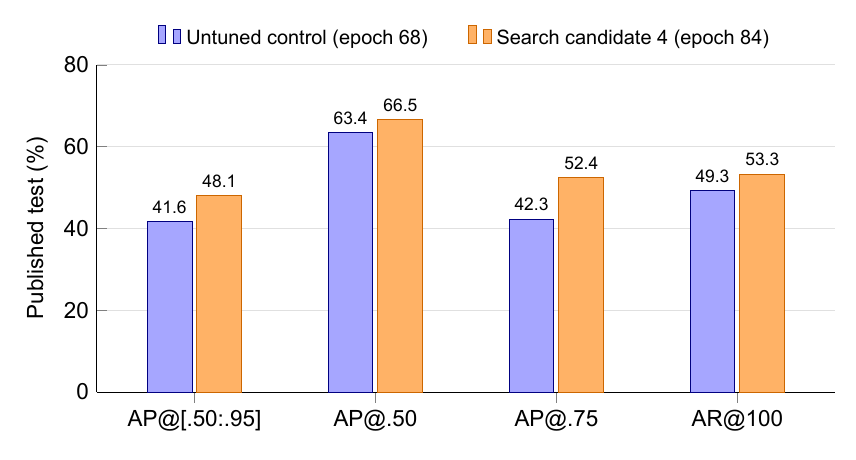
\includegraphics[width=0.9\textwidth]{t41-test.png}
\caption{Test COCO metrics of the control and the candidate.}
\label{fig:t41test}
\floatnote{Published test set; both models were trained for up to 100 epochs from the same starting weights.}
\end{figure}

\begin{figure}[htbp]\centering
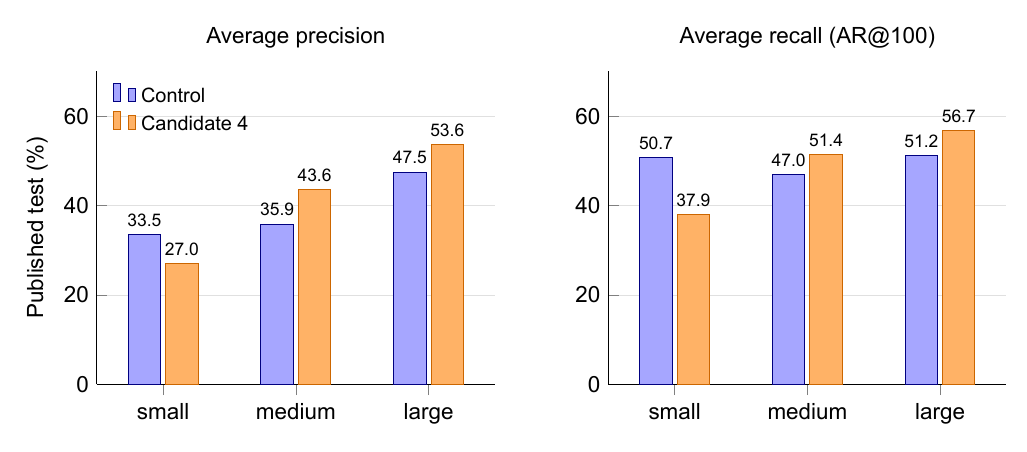
\includegraphics[width=\textwidth]{t41-size.png}
\caption{Test AP and AR by object size.}
\label{fig:t41size}
\floatnote{COCO object sizes on the published test set. The candidate is better on medium and large objects and worse on small ones.}
\end{figure}

The candidate scored 6.46 percentage points higher test AP than the control, with
the largest gain at the stricter IoU of 0.75, which indicates tighter boxes. It
was, however, worse on small objects (AP 27.05\% against 33.49\%, AR 37.89\%
against 50.70\%). Because the candidate was chosen on validation, where it was
slightly worse, the test difference describes this one pair of models; it does
not justify selecting a deployment model after seeing the test scores.

Figure~\ref{fig:t41pr} shows the precision--recall curves behind these AP values,
recomputed from the saved predictions; their averages reproduce AP@.50 and
AP@.75 exactly. At IoU~0.50 the candidate's curve lies above the control's over
almost the whole range, keeping precision above 90\% up to a recall of 0.56
against 0.48 for the control. Both curves end at a recall of 0.70: even at the
lowest score kept (0.001), about 30\% of the annotated threats receive no
matching detection, so lowering the threshold cannot recover them. At the
stricter IoU~0.75 the maximum recall falls to 0.51 and 0.58, which shows that
many detections are found but poorly localized.

\begin{figure}[htbp]\centering
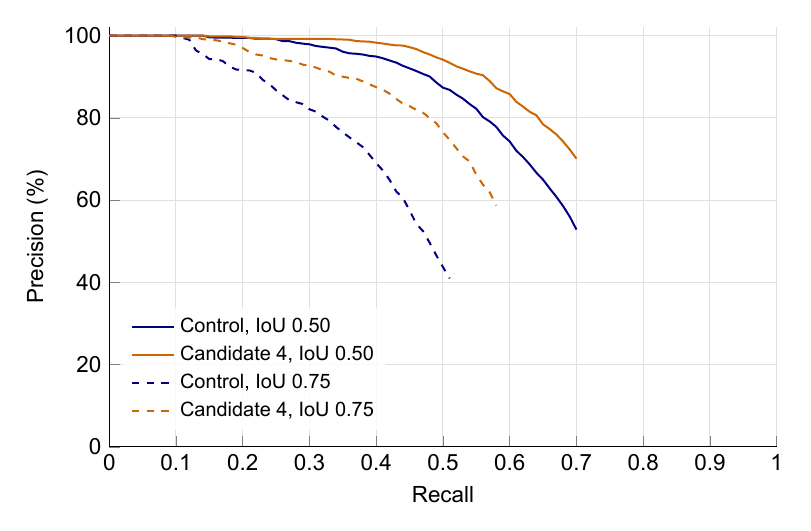
\includegraphics[width=0.85\textwidth]{t41-pr.png}
\caption{Precision--recall curves on the test set.}
\label{fig:t41pr}
\floatnote{IoU 0.50 (solid) and 0.75 (dashed), computed with pycocotools from the saved predictions of job 820. Curves end at the highest recall each model reaches.}
\end{figure}

\subsection{Fixed Operating Point}
An operator sees detections above a confidence threshold, not an AP value. A
threshold of 0.25 with matching at IoU~0.50 was fixed before the test as an
illustrative operating point; it is not optimized or safety-qualified.
Figure~\ref{fig:t41op} and Table~\ref{tab:t41op} show the counts.

\begin{table}[htbp]
\centering\tablesetup
\caption{Detection counts at the fixed operating point.}
\label{tab:t41op}
\begin{tabular}{@{}lrr@{}}
\toprule
Quantity & Untuned control & Candidate 4\\
\midrule
True positives & 1,562 & 1,547\\
False positives & 193 & 80\\
Missed annotated boxes & 1,642 & 1,657\\
False positives on images with no annotation & 55 & 25\\
Precision (\%) & 89.00 & 95.08\\
Recall (\%) & 48.75 & 48.28\\
\bottomrule
\end{tabular}
\floatnote{Confidence 0.25 and IoU 0.50 on the published test set (3,204 annotated boxes).}
\end{table}

\begin{figure}[htbp]\centering
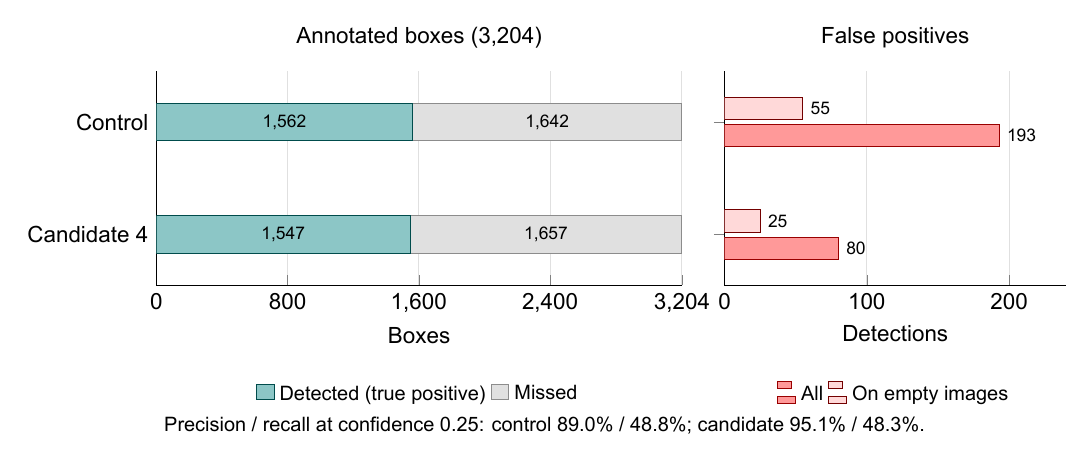
\includegraphics[width=\textwidth]{t41-oppoint.png}
\caption{Detected, missed and false boxes at the operating point.}
\label{fig:t41op}
\floatnote{Left: detected and missed annotated boxes. Right: false positives.}
\end{figure}

At this threshold the candidate produced 59\% fewer false positives, raising
precision from 89.0\% to 95.1\%, but both models detected fewer than half of the
annotated explosives. For a screening aid, a recall below 49\% is the most
important limitation of the prototype: a missed threat is far more costly than a
false alarm that an operator can dismiss. A lower threshold would trade
precision for recall, and choosing it requires a calibration set that is not the
test set.

\subsection{Inspected Examples}
After the evaluation, three test images and their saved predictions were inspected
without changing any model or setting. The selection was descriptive: the first
missed image in order, the candidate's highest-scoring false positive, and an
image already flagged during the audit.
\begin{itemize}
\item \file{Test000001.jpg}: the annotated threat lies over a dense electronic
region. Both models miss it at 0.25; the control's best score is 0.033, and the
candidate produces no detection even at 0.001.
\item \file{Test004918.jpg}: the candidate predicts a region with score 0.945, but
the generic annotation file has no box for this image. It counts as a false
positive against that file; the image is not thereby certified as benign.
\item \file{Test000071.jpg}: the image with the open question over its modified
host label. Both scores are below 0.25 (0.017 and 0.001).
\end{itemize}
Figure~\ref{fig:t41examples} shows the three images with the annotated box and
the models' detections.

\begin{figure}[htbp]\centering
\IfFileExists{figures/private/t41-ex-miss.png}{%
\includegraphics[width=\textwidth]{private/t41-ex-miss.png}\\[2pt]
{\small (a) \file{Test000001.jpg}: missed threat}\\[6pt]
\includegraphics[width=\textwidth]{private/t41-ex-false-positive.png}\\[2pt]
{\small (b) \file{Test004918.jpg}: detection with no annotation}\\[6pt]
\includegraphics[width=\textwidth]{private/t41-ex-label-question.png}\\[2pt]
{\small (c) \file{Test000071.jpg}: open label question}}{%
\fbox{\parbox{0.9\textwidth}{\centering\small The annotated test images are kept
outside the repository. Build them with \file{docs/report/tools/t41_figures.py}
(see \file{docs/report/README.md}).}}}
\caption{Inspected test images.}
\label{fig:t41examples}
\floatnote{Untuned control (left) and candidate~4 (right). Magenta: annotated threat; blue or orange: detection at confidence $\geq 0.25$; grey: the model's highest-scoring detection below 0.25, with its score. Images from the published IEDXray test set~\citep{takele2026iedxray}, reproduced with attribution; overlays added by the team.}
\end{figure}

\subsection{Latency and Resources}
Table~\ref{tab:t41latency} reports inference time on the H100 NVL with batch size
one and FP32, after five warm-up images from the validation set. The predictor
time includes image loading, pre-processing, the model and post-processing; it
excludes input hashing and record writing. At about 7.4~ms per image the
detector is fast enough for interactive use, although the complete operator
workflow, the interface and the scanner hand-off were not timed. The peak GPU
memory allocated by the inference process was 233~MB for the control and
301~MB for the candidate.

\begin{table}[htbp]
\centering\tablesetup
\caption{Inference time per image.}
\label{tab:t41latency}
\begin{tabular}{@{}lrrrr@{}}
\toprule
& \multicolumn{2}{c}{Untuned control} & \multicolumn{2}{c}{Candidate 4}\\
\cmidrule(lr){2-3}\cmidrule(l){4-5}
Timing boundary & Median & p95 & Median & p95\\
\midrule
Predictor call (end to end) & 7.395 & 8.086 & 7.387 & 7.886\\
Model inference only & 5.589 & 5.713 & 5.583 & 5.691\\
\bottomrule
\end{tabular}
\floatnote{Published test set, 5,136 images per model; milliseconds.}
\end{table}

\subsection{Discussion and Limitations}
The prototype detects concealed explosives with moderate accuracy: about half of
the annotated threats are found at the fixed threshold, and the boxes it does
produce are mostly correct. Figure~\ref{fig:t41gap} shows the most important
caveat. Both models scored about 87.5\% AP on the validation set but 41.6\% and
48.1\% on the published test set, a gap of 46.1 and 39.4 percentage points. The validation images come from the same
training split, and without verified physical groups, near-identical scans of the
same bag can appear on both sides of the fit/validation partition, which inflates
validation scores. Four exact-byte overlaps between the published training and
test sets and 112 duplicate pairs inside the test set were deliberately retained
to keep the published split intact. The test score is therefore the more
realistic estimate, but it is not an unseen-case benchmark.

\begin{figure}[htbp]\centering
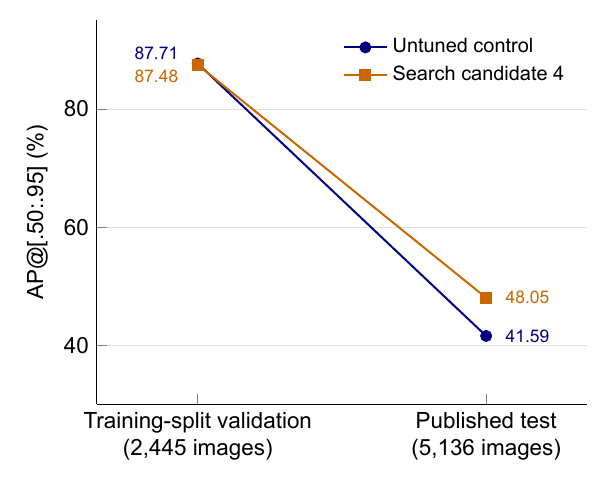
\includegraphics[width=0.62\textwidth]{t41-gap.png}
\caption{Validation and test AP of both models.}
\label{fig:t41gap}
\floatnote{The gaps of 46.1 (untuned) and 39.4 (tuned) percentage points indicate optimistic validation on a split without verified physical groups.}
\end{figure}

The remaining limits follow from the reduced scope. Only one training seed was
used, so no statistical significance or repeatability is claimed. The
specific-explosive task, the full 20-attempt search and the multi-seed study were
deferred. The results concern single-scan generic detection and do not evaluate
host association or threats distributed across several bags. These experiments are
planned for SDP~II (Section~\ref{sec:further}).
\projectrecord{docs/t41-results.md}

%-----------------------------------------------------------------------------
\section{Application Walkthrough}\label{sec:walkthrough}
This section follows one scan through RayGuard-App, from setup to a saved review. The
screenshots were captured on 24~November~2026 from real runs of the application
(application code at revision \file{3488abd}, engine \file{b7ec59e}) on a CPU, at the
fixed threshold of 25\%. Each run took about 12--17~seconds, including the start of the
model process. The scans come from the published IEDXray test
set~\citep{takele2026iedxray}, reproduced with attribution.

\textbf{Model shown.} The screenshots use the YOLOv10-M checkpoints supplied with
IEDXray, not the detector fine-tuned in Section~\ref{sec:results}. The generic
checkpoint has the same architecture, task and output class as the fine-tuned model,
whose weights are not yet integrated in the application. The walkthrough demonstrates
the application and is not evidence of accuracy. The scans were chosen after running
the supplied models on 260 annotated and 60 unannotated test images: two clear
detections, one image without an annotated threat, and the missed threat already shown
in Figure~\ref{fig:t41examples}. None of the four has an exact copy in the training set.

\subsection{Inspecting One Scan}
\begin{enumerate}
\item \textbf{Set up.} The operator chooses an input workflow and a model. The page
shows the model classes, the device and the threshold (Figure~\ref{fig:appsteps}a).
\item \textbf{Load.} A bag scan is uploaded and shown before any detection. Viewing
adjustments change the display only (Figure~\ref{fig:appsteps}b).
\item \textbf{Run.} The operator starts inference explicitly. The scan being processed
is kept apart from the latest completed result (Figure~\ref{fig:appsteps}c).
\item \textbf{Inspect.} The detector marks one region inside the laptop with a score of
91.6\%, linked to its entry in the findings list (Figure~\ref{fig:appresult}).
\item \textbf{Trace.} The provenance tab records the run, threshold, task and checkpoint
hash (Figure~\ref{fig:appsteps}d).
\item \textbf{Review.} The operator adds a note and flags the scan for follow-up. The
application states that a review does not clear or classify the item
(Figure~\ref{fig:appsteps}e).
\item \textbf{Record.} The session page lists every run with its status and review, and
each run can be exported as JSON (Figure~\ref{fig:appsteps}f).
\end{enumerate}

\begin{figure}[htbp]\centering
\IfFileExists{figures/private/app-result.png}{%
\includegraphics[width=\textwidth]{private/app-result.png}}{%
\fbox{\parbox{0.9\textwidth}{\centering\small Screenshots showing dataset scans are kept
outside the repository (see \file{docs/report/README.md}).}}}
\caption{Detection result in RayGuard-App.}
\label{fig:appresult}
\floatnote{IEDXray scan \file{Test001489}~\citep{takele2026iedxray}: one region localized inside the laptop by the supplied generic-explosive checkpoint. The score is not a calibrated probability.}
\end{figure}

\begin{figure}[htbp]\centering
\IfFileExists{figures/private/app-steps.png}{%
\includegraphics[width=\textwidth]{private/app-steps.png}}{%
\fbox{\parbox{0.9\textwidth}{\centering\small Screenshots showing dataset scans are kept
outside the repository (see \file{docs/report/README.md}).}}}
\caption{Walkthrough of one scan.}
\label{fig:appsteps}
\floatnote{(a) Workspace setup, (b) scan loaded, (c) inference running, (d) provenance with checkpoint hash, (e) operator review flagged for follow-up, (f) session records. Supplied generic checkpoint; the navigation sidebar is cropped.}
\end{figure}

\subsection{Comparison with the Reference and Other Tasks}
In dataset replay, the application compares a saved generic result with the published
annotation. Figure~\ref{fig:appcompare} shows two matched threats, an image without an
annotated target and a missed threat. The last two are displayed with the message that an
empty result is not a safety verdict. Table~\ref{tab:appcases} adds the fine-tuned models'
results for the same scans, taken from the saved predictions of job~820 and not produced in
the application. The fine-tuned candidate also finds the laptop threat, but it misses the
walkie-talkie threat that the supplied model finds.

\begin{table}[htbp]
\centering\tablesetup
\caption{Matching scores on the walkthrough scans.}
\label{tab:appcases}
\begin{tabularx}{\textwidth}{@{}L{0.17\textwidth}YL{0.17\textwidth}L{0.15\textwidth}L{0.15\textwidth}@{}}
\toprule
Scan & Content & Supplied model (application) & Control (job 820) & Candidate (job 820)\\
\midrule
\file{Test001489} & Annotated threat in a laptop & 0.916 & 0.968 & 0.954\\
\file{Test002804} & Annotated threat in a walkie-talkie & 0.899 & 0.525 & none (best 0.137)\\
\file{Test003370} & Laptop, no annotated threat & no detection & no detection & no detection\\
\file{Test000001} & Annotated threat over electronics & none & none & none\\
\bottomrule
\end{tabularx}
\floatnote{Highest score at or above 0.25 that matches the annotation with IoU $\geq$ 0.5. Four selected images; not a comparison of model accuracy.}
\end{table}

\begin{figure}[htbp]\centering
\IfFileExists{figures/private/app-compare.png}{%
\includegraphics[width=\textwidth]{private/app-compare.png}}{%
\fbox{\parbox{0.9\textwidth}{\centering\small Screenshots showing dataset scans are kept
outside the repository (see \file{docs/report/README.md}).}}}
\caption{Comparison with the published annotation.}
\label{fig:appcompare}
\floatnote{Annotation in dashed cyan, supplied generic checkpoint in amber: (a) matched threat in a laptop, (b) matched threat in a walkie-talkie, (c) no annotated target and no detection, (d) missed threat.}
\end{figure}

The same scan can be examined with the other supplied tasks
(Figure~\ref{fig:appmodels}). The device model localizes the laptop (91.5\%) and the
specific-explosive model labels the region as a laptop explosive (98.3\%). Both models
passed the application's execution check before use. The application keeps the three
tasks separate and does not combine them into a decision.

\begin{figure}[htbp]\centering
\IfFileExists{figures/private/app-models.png}{%
\includegraphics[width=\textwidth]{private/app-models.png}}{%
\fbox{\parbox{0.9\textwidth}{\centering\small Screenshots showing dataset scans are kept
outside the repository (see \file{docs/report/README.md}).}}}
\caption{One scan with the other supplied checkpoints.}
\label{fig:appmodels}
\floatnote{Scan \file{Test001489}: (a) device detection, (b) specific-explosive detection. Supplied IEDXray checkpoints.}
\end{figure}

\subsection{Interface Evidence from T43}
The interface behaviour around these steps, such as failed runs, filters, unsaved notes
and accessibility, is covered by the eight acceptance tests of RayGuard-App PR~\#1. They
use synthetic images and do not involve a model.

%-----------------------------------------------------------------------------
\section{Application Acceptance}\label{sec:acceptance}
The application is accepted for the demonstration after a dated human rehearsal on
the presentation machine, recording the application and engine revisions. The
rehearsal covers:
\begin{enumerate}
\item a clean start of the application;
\item loading an authorized input image;
\item selecting a model task and obtaining real localizations;
\item reviewing the findings and exporting the record;
\item demonstrating a known miss or error state.
\end{enumerate}
Any pre-recorded fallback must be labelled as recorded. The hand-off of images from
the scanner export and the current application revision also require a dated
acceptance record. No new feature is needed only to generate contribution evidence.

The walkthrough with the fine-tuned checkpoint and a current end-to-end rehearsal remain
open at the date of this report.

\chapter{Conclusions}\label{ch:conclusions}
\section{Summary of work}
RayGuard has a concrete single-scan prototype path and a growing research
software foundation. Audits, strict contracts and bounded real execution
support image-to-result integration. The separate application exposes localized
findings and traceable operator review. Evaluation and initialization software
have been integrated. The reduced generic study completed six attempted
configurations, two 100-epoch confirmations and a frozen full published-test
comparison, with saved predictions and independently recomputed metrics.

\section{Critical appraisal}
The current evidence includes reproducible software checks and measured generic
detector performance, with a substantial validation-to-test AP gap. The dataset audits reveal why broad accuracy
or unseen-data claims require care: task exports disagree, exact images cross
the supplied split, boundary findings remain, and physical groups are not
established locally. The collection inventory is useful progress evidence,
but it does not yet establish independent labeled cases or accepted completion.

The project has not demonstrated full P1 host/threat decisions, distributed-case
fusion, a live scanner connection or repeatable benchmark improvement. The
preselected candidate achieved higher test AP in one run, but lower small-object
AP and fixed-threshold recall; both models missed roughly half the annotated
boxes at confidence 0.25. These
limits affect the system's permitted interpretation. An operator should not
treat an empty detector output as clearance, nor a plausible component grouping
as proof of a functional device. Explicit states and provenance help communicate
these limits but cannot replace performance and safety validation.

\section{Further work}
The immediate handoff is review of the qualified implementation, frozen results
and report evidence. No additional training is needed to finish the authorized
deadline scope. Future experiments should establish physical groups and assess
repeatability on training-derived validation before any new final test protocol.
The deferred specific-task and original twenty-attempt studies must not be
reported as completed. The report deadline remains 24 November 2026 at
17:00 UTC+4; the completed generic results and their limitations support the
23 November evidence freeze.

The longer-term distributed work requires QC, accepted collection counts,
component annotations, physical/case provenance and a case-disjoint evaluation
design. A transparent independent-scan aggregation baseline should be assessed
before introducing learned fusion, provided suitable ground truth exists.
Human acceptance on the presentation machine and an observed scanner handoff
remain separate deployment steps. The overall collection deadline of
30 November is retained independently of report submission.

The completed report should explain both the achieved prototype and the work
still necessary to justify stronger claims. Its final contribution table,
forms and conclusions require student and supervisor review.

\bibliographystyle{IEEEtran}
\bibliography{references}
\appendix
\chapter{Project Management}\label{app:management}
\section{Schedule and dependencies}
Figure~\ref{fig:gantt} separates recorded semester evidence from
forward delivery work. A marker indicates an
event or evidence date, not continuous effort or completed hours. Earlier
8/15 October prototype targets are retained as historical obligations; they
are not silently replaced by the November plan.

\begin{figure}[htbp]\centering
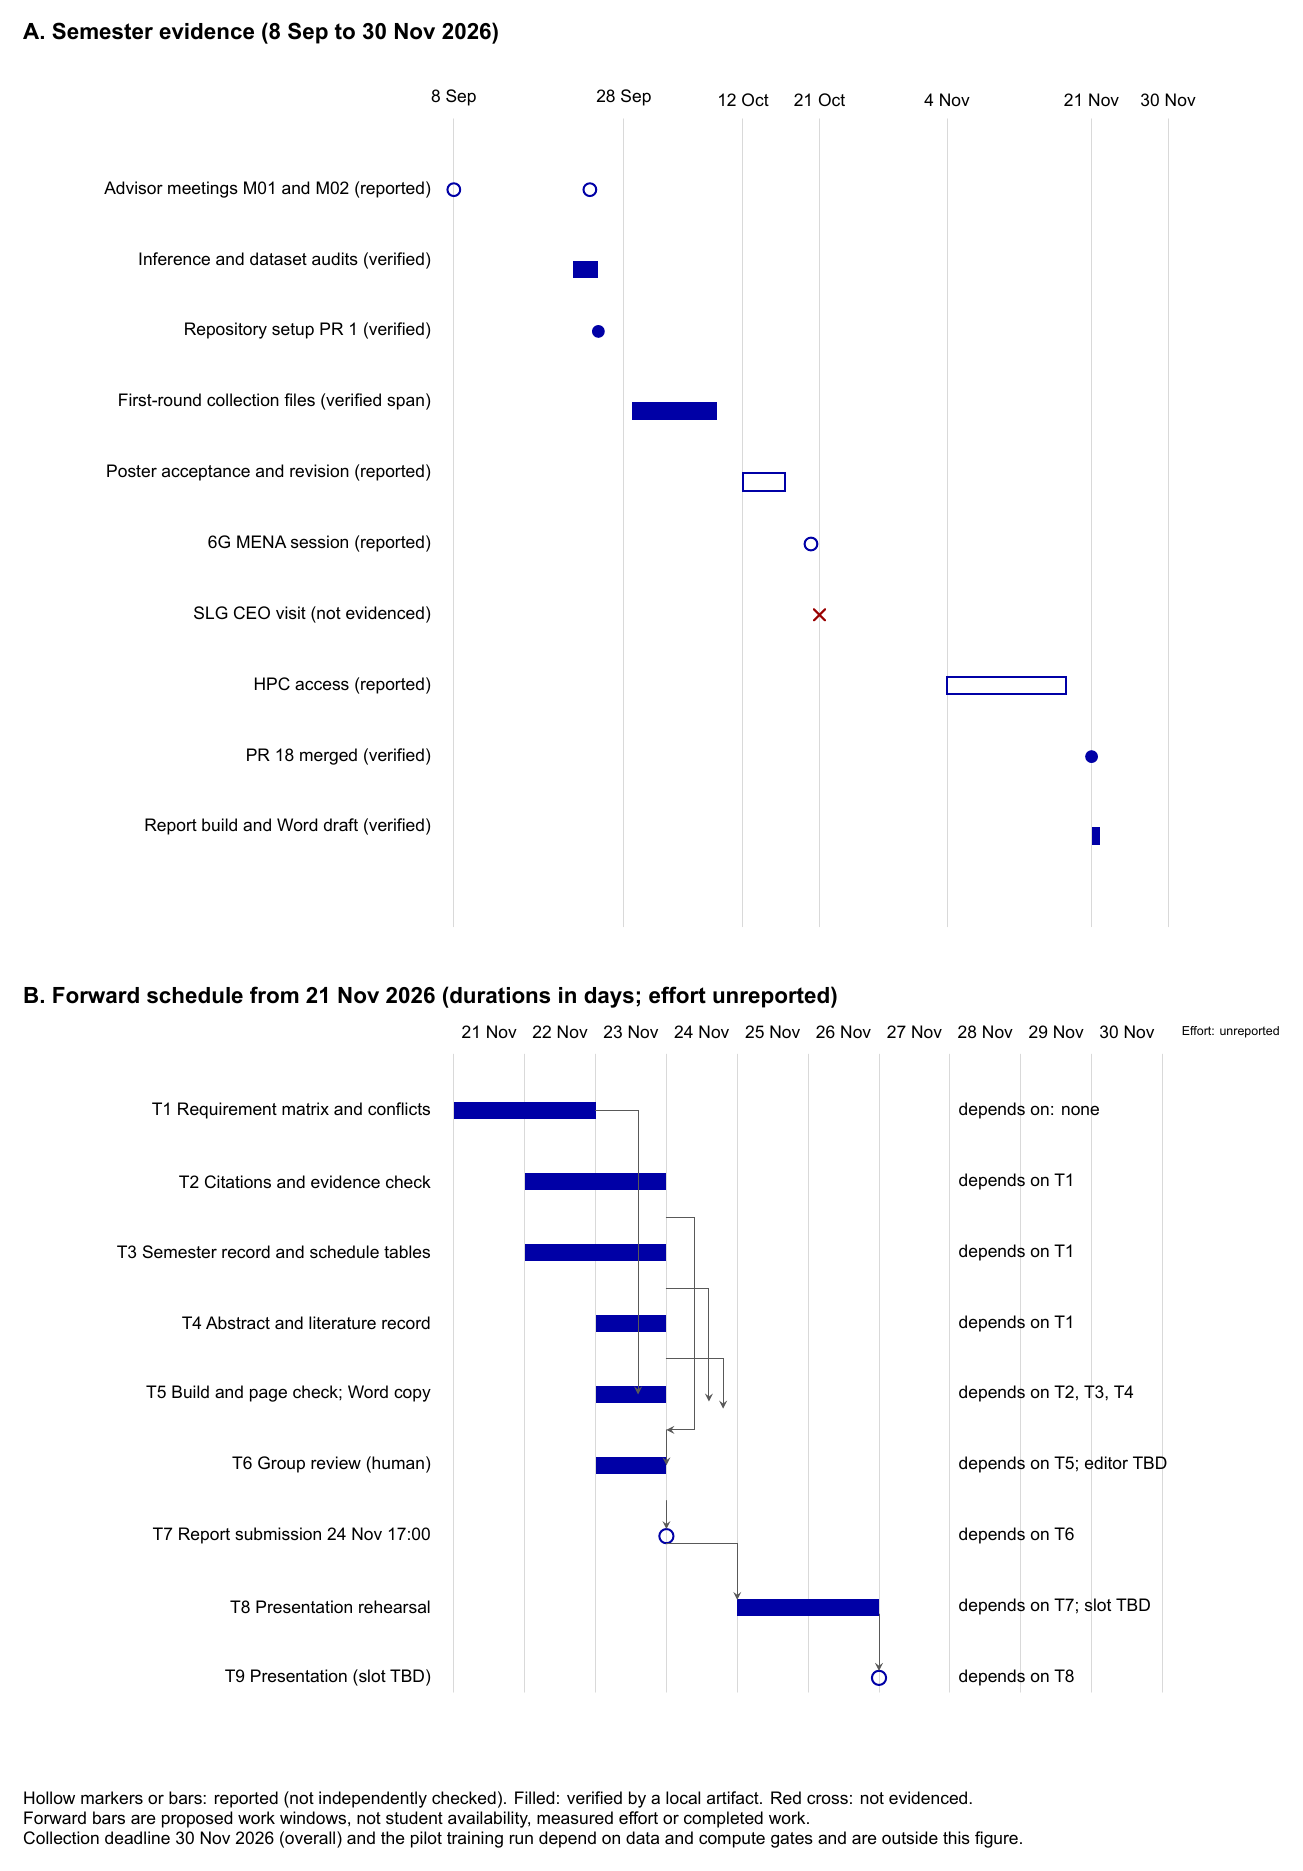
\includegraphics[width=\textwidth]{gantt.png}
\caption{Schedule summary in two panels. Panel A places recorded semester events by evidence status: filled markers are verified, hollow markers are reported and not independently checked, and the red cross is not evidenced. Panel B gives the forward schedule from 21 November 2026 with durations, dependencies and responsibilities. Effort is unreported for every task, and no bar measures student effort.}
\label{fig:gantt}
\end{figure}

\begingroup\small
\begin{longtable}{p{0.21\textwidth}p{0.34\textwidth}p{0.35\textwidth}}
\caption{Dependencies and contingencies for the final SDP I delivery.}\\
\toprule Deliverable & Required dependency & Contingency or open action\\\midrule\endfirsthead
\toprule Deliverable & Required dependency & Contingency or open action\\\midrule\endhead
Training pilot & Reviewed data receipts, actual initialization and qualified backend & Report software preparation and precise blockers if execution cannot qualify\\
Real evaluation & Matching predictions/ground truth and frozen protocol & Keep results explicitly unavailable; never substitute paper or synthetic scores\\
Demo & Current machine, engine/model identity and authorized examples & Clearly labeled saved real-run fallback, with known failures retained\\
Report & Verified evidence, reference review, forms and student contribution statements & Freeze factual content for 23 Nov review; retain explicit limitations\\
Submission & Active Blackboard format, project number, actual signatures and distribution clearance & Checked Word copy alongside LaTeX PDF; confirm institutional instructions before upload\\
Distributed work & QC, accepted counts, labels and physical/case grouping & Preserve 30 Nov collection obligation; do not infer P2 completion\\\bottomrule
\end{longtable}
\endgroup

Task names identify coordination contacts, not exclusive rights to files.
Students prioritize assigned work and may complete a small dependency that
blocks it without waiting for its lead. They record actual editor/scope and
coordinate overlapping active edits or GPU/output use. Independent review
and truthful credit remain necessary. The sole live backlog is
\file{docs/tasks.md}; this appendix is a dated summary.

\section{Semester record}
Table~\ref{tab:record} lists events and milestones from September to November 2026.
Each row states its evidence status. \emph{Verified} means a local artifact, repository
state or read-back confirms it. \emph{Reported} means an owner statement, email or meeting
record that has not been independently checked. Conflicts are listed in
Table~\ref{tab:conflicts} and are not resolved here.

\begingroup\small
\begin{longtable}{>{\raggedright\arraybackslash}p{0.14\textwidth}>{\raggedright\arraybackslash}p{0.36\textwidth}>{\raggedright\arraybackslash}p{0.22\textwidth}>{\raggedright\arraybackslash}p{0.18\textwidth}}
\caption{Dated semester record, September to November 2026.}\label{tab:record}\\
\toprule Date & Event & Outcome & Evidence\\\midrule\endfirsthead
\toprule Date & Event & Outcome & Evidence\\\midrule\endhead
8 Sep 2026 & Advisor meeting M01 (Prof.\ Werghi) & Source minutes and companion; attendance not confirmed & Reported\\
22--25 Sep & Generic inference and dataset audits & Generic inference ran; device-label and split findings recorded & Verified\\
24 Sep & Advisor meeting M02; Divya follow-up F02 & Batch 1 by 15 Oct, Batch 2 after midterms, GUI and poster tasks & Reported (minutes hash verified)\\
25 Sep & Team repository setup (PR \#1, rulesets) & Published; hosted checks passed & Verified\\
28 Sep & Collection emails F03--F05; catalogue C01 & Revised slots 29 Sep--8 Oct; catalogue structure checked & Reported; catalogue verified\\
29 Sep--9 Oct & First-round collection files (filename span only) & 577 JPEG paths, 478 distinct payloads, all decode & Verified (files); sessions reported\\
12--17 Oct & Poster acceptance and revision & Accepted 12 Oct; revised file 17 Oct; TDRA response pending & Reported\\
19 Oct & Collection update F06; SLG visit invitation F08 & 30 Nov overall deadline; visit 21 Oct, 14:00--17:00 & Reported (invitation only)\\
20 Oct & 6G MENA session, Abu Dhabi & Team attendance owner-reported; presentation evidence not reviewed & Reported\\
21 Oct & SLG CEO visit & No outcome recorded in the project record & Not evidenced\\
4--18 Nov & CS-HPC access email; owner confirmation & Access issued; training run not verified & Reported\\
21 Nov & PR \#18 merged (commit 9350482) & 273 evaluation-enabled tests and required CI passed & Verified\\
21 Nov & Report LaTeX build and Word draft & Local build passes; Word layout review open & Verified (local)\\bottomrule
\end{longtable}
\endgroup

\textbf{Conferences and events.} The project record lists the ISDIA and ICISAS calls
(closed 15 November 2026, no submission recorded), the CVCI call (official deadline
30 November 2026, conflicting with a 5 December invitation) and a ZU SRC abstract window
(15 December 2026 to 18 January 2027). No submission or acceptance for any event is recorded.

\begingroup\small
\begin{longtable}{>{\raggedright\arraybackslash}p{0.44\textwidth}>{\raggedright\arraybackslash}p{0.52\textwidth}}
\caption{Open conflicts recorded in the project, not resolved in this report.}\label{tab:conflicts}\\
\toprule Item & Conflict\\\midrule\endfirsthead
\toprule Item & Conflict\\\midrule\endhead
Report deadline & 24 Nov 2026, 17:00 UTC+4 (owner) versus 27 Nov 2026 (pasted notice)\\
Collection deadline & Batch 1 by 15 Oct (historical) versus 30 Nov overall\\
Collection count & Target 500 versus 577 paths and 478 distinct payloads\\
Round 1 allocation & One item per student (F03) versus all four families per student (C01)\\
PR \#21 status & Recorded as merged in one task row and open in the status record\\
Logo adoption & A04 in one progress heading versus A03 approved 28 Sep in the status record\\
Poster timeline & 30 Sep, 14 Oct, 17 Oct revision versus 20 Oct confirmation\\
\bottomrule
\end{longtable}
\endgroup

\section{Handbook-form task schedule}
Table~\ref{tab:tasks} sets out the schedule elements the handbook asks for. Effort in hours
was not recorded for any task, so the effort column reads ``unreported'' rather than an estimate.
Durations are the dates in the project record, not measured effort.

\begingroup\small
\begin{longtable}{>{\raggedright\arraybackslash}p{0.22\textwidth}>{\raggedright\arraybackslash}p{0.10\textwidth}>{\raggedright\arraybackslash}p{0.12\textwidth}>{\raggedright\arraybackslash}p{0.26\textwidth}>{\raggedright\arraybackslash}p{0.22\textwidth}}
\caption{Task schedule in handbook form (effort unreported).}\label{tab:tasks}\\
\toprule Task & Duration & Effort & Depends on & Output and contingency\\\midrule\endfirsthead
\toprule Task & Duration & Effort & Depends on & Output and contingency\\\midrule\endhead
Report drafting (LaTeX, bibliography) & 21--24 Nov & unreported & Verified evidence; references & Build and PDF; contingency: freeze content for review\\
Group review and Word copy & 23--24 Nov & unreported & Build; Pandoc conversion & Word draft; contingency: PDF if accepted\\
Presentation rehearsal & 25--26 Nov & unreported & Demo candidate; slot & Rehearsed demo; contingency: recorded fallback\\
Presentation & 27 Nov (stated) & unreported & Slot confirmation & Presentation; slot TBD\\
Collection completion & to 30 Nov & unreported & Lab protocol; QC & Accepted counts; open conflict in Table~\ref{tab:conflicts}\\
Pilot training and evaluation & after data gates & unreported & Data receipts; qualified runtime & Not started; no results claimed\\bottomrule
\end{longtable}
\endgroup

\chapter{Risk and Required Forms}\label{app:risk}
\section{Risk preparation worksheet}
Table~\ref{tab:risk} is a draft engineering worksheet for discussion, not the
official completed Risk Assessment or Health and Safety form. Likelihood,
severity, residual ratings and named signatories require supervisor/lab review.
No signature, approval or absence of hazards is inferred here.

\begingroup\small
\begin{longtable}{p{0.2\textwidth}p{0.32\textwidth}p{0.38\textwidth}}
\caption{Draft hazard and project-risk discussion worksheet.}\label{tab:risk}\\
\toprule Hazard or risk & Possible consequence & Proposed controls and outstanding review\\\midrule\endfirsthead
\toprule Hazard or risk & Possible consequence & Proposed controls and outstanding review\\\midrule\endhead
Lab X-ray equipment & Exposure or unsafe operation & Trained authorized operation, intact interlocks and lab procedures; lab/supervisor determines applicable radiation controls\\
Electrical equipment and specimen handling & Injury, damage or unapproved operation & Follow lab-approved equipment/specimen protocol; no unsupervised hazardous work; confirm permitted inert materials with lab\\
Missed detections or overconfidence & Incorrect inspection decision & Human review, known-miss demonstration, visible failure states and no safe verdict from empty results\\
Data and credentials & Disclosure or unauthorized access & Authorized local storage, sanitized exports, no scans/weights/credentials/private paths in public Git\\
Split leakage and invalid labels & Misleading evaluation or tuning & Preserve published test, hash artifacts, group duplicates, review geometry and physical provenance; no test-based tuning\\
Compute failure or excess resource use & Lost study evidence, missed deadline or quota breach & One job/output owner, checkpoint/restart evidence, bounded pilot and measured budget before search\\
Software mismatch & Invalid result or demo failure & Pinned environments, actual device/revision records, clean startup checks and labeled recorded fallback\\
Contribution and AI attribution & Misrepresentation in individual assessment & Actual work links, student explain-back and truthful assistance disclosure; no invented hours\\
Report and publication & Rejected submission or confidential disclosure & Confirm Word/PDF acceptance and filename; actual form signatures; resolve written-permission requirement before public distribution\\\bottomrule
\end{longtable}
\endgroup

\section{Official form insertion checklist}
The handbook lists Risk Assessment and Health and Safety forms for SDP I/II.
Its Health and Safety form calls for student representative and supervisor
signatures and handling by the University Safety Officer. Confirm the current
course templates and insert their completed, authorized copies into the
submission version. Do not mark the project software-only without reviewing
the team's physical lab collection work.

\pending{Official Risk Assessment form, completed Health and Safety form,
current declaration wording, actual signatures, recipients and dates. The
current draft intentionally contains no fabricated declaration or signature.}

The Project Clearance I/II forms are explicitly marked for the SDP II final
report. They are not treated as new SDP I submission requirements without
a specific course instruction. Physical final-copy requirements and public
distribution remain to be clarified against the later course notices.

\chapter{Contribution and Assistance Record}\label{app:contributions}
The entries below distinguish repository evidence from personal understanding.
They are draft source records for student confirmation, not a final allocation
of marks or hours. Team names follow shared records and require roster confirmation.

\begingroup\small
\begin{longtable}{p{0.19\textwidth}p{0.41\textwidth}p{0.3\textwidth}}
\caption{Evidence-linked contribution worksheet for individual confirmation.}\\
\toprule Student & Existing source record & Verification still needed\\\midrule\endfirsthead
\toprule Student & Existing source record & Verification still needed\\\midrule\endhead
Abd Alrahman Ismaik & Coordination/GUI direction recorded in project documentation; assisted integration and report preparation & Personal reviewed contribution statement, report sections and explain-back\\
Faisal Daoud Alzarooni & T40 baseline/contracts/tools PRs 17/19; initialization PR 21 & Student confirmation, actual HPC handoff and explain-back\\
Ahmed Almansoori & T41 branch commit 32091bc; pipeline checks, planning and synthetic study draft & Student confirmation and integration evidence; real training not yet established\\
Ali Arif Alshamsi & T42 evaluator PR 18, validation interface and matched comparison & Student confirmation, real evaluation evidence when available and explain-back\\
Mohammad Arwani & Research branch records an assisted app acceptance slice & Verified shared app commit/diff, human walkthrough and roster spelling\\\bottomrule
\end{longtable}
\endgroup

AI assistance was used in implementation, review and documentation preparation,
including this report draft. Each student must review and understand the work
they claim. Relevant sanitized code-generation prompts and assistance details
must be included accurately in the final disclosure; private transcripts,
credentials and session records remain outside the public repository.
\pending{Student-reviewed disclosure and relevant sanitized prompt excerpts.}

\chapter{Handbook Coverage and Source Map}\label{app:coverage}
\begingroup\small
\begin{longtable}{p{0.12\textwidth}p{0.45\textwidth}p{0.33\textwidth}}
\caption{R01--R15 traceability for this draft. Presence is not final acceptance.}\\
\toprule ID & Draft location & Remaining gate\\\midrule\endfirsthead
\toprule ID & Draft location & Remaining gate\\\midrule\endhead
R01 & Cover, abstract, contents and lists & Institutional cover/roster confirmation\\
R02 & Chapter 1 objectives and scope & Student/supervisor review\\
R03 & Chapter 1 literature & Deeper reference reading; scoped patent-search record\\
R04 & Chapter 1 and Appendix C & Individual confirmations and sanitized prompts\\
R05 & Chapter 2, Table 2.1 & Formal requirements/specification review\\
R06 & Chapter 3 & Technical review of assumptions and equations\\
R07 & Chapter 4 & Final design rationale review\\
R08 & Chapter 5 & Current app revision and approved screenshots\\
R09 & Chapter 5 & Eligible real metrics and demonstration evidence\\
R10 & Chapter 6 & Conclusions updated to final evidence cutoff\\
R11 & References & Verify relevance, metadata and final citation coverage\\
R12 & Appendix A and original specification below & Gantt actuals/student ownership confirmation\\
R13 & Appendix B & Official completed forms and actual signatures\\
R14 & Appendix B & Official declaration and applicable paperwork\\
R15 & Project course checklist & Actual submission, permission and rehearsal receipts\\\bottomrule
\end{longtable}
\endgroup

\section{Original specification summary}
The original proposal requires image acquisition of 500 positive/negative
samples; preprocessing for image quality; contemporary explosive detection;
evaluation on unseen test data; and a GUI supporting control and recording.
This summary preserves the requirements without reproducing private source
documents. Later meetings prioritize distributed collection and retain a
single-scan existing-model showcase. Table~\ref{tab:requirements} maps the
current implementation without treating later planning as waiver of older
requirements.

\section{Project source register}
\begingroup\small
\begin{longtable}{p{0.4\textwidth}p{0.5\textwidth}}
\caption{Project records supporting the report; paths are repository-relative.}\\
\toprule Source record & Use and evidence boundary\\\midrule\endfirsthead
\toprule Source record & Use and evidence boundary\\\midrule\endhead
\file{docs/final-report-requirements.md} & Handbook requirements and R01--R15; original handbook remains local\\
\file{docs/meeting_minutes/README.md} & M01/M02 and F02--F08 directions; minutes do not prove execution\\
\file{docs/research.md} & Paper and release inspection; published claims remain distinct\\
\file{docs/iedxray-audit.md} & Audit findings and source preservation\\
\file{docs/first-inference.md} & Initial executed CPU diagnostic inference and retained miss\\
\file{docs/architecture.md} & Contract and repository boundary; older passages require revision-aware reading\\
\file{docs/collection-progress-2026-11-14.md} & Path/byte inventory and unresolved QC/provenance\\
\file{docs/progress.md} & Dated integration commands, test outcomes and limitations\\
\file{docs/course-endgame-2026-11.md} & Submission/presentation notices and conflicts\\
\file{docs/tasks.md} & Sole live backlog; this report is a dated evidence snapshot\\\bottomrule
\end{longtable}
\endgroup

\end{document}
